%%%%%%%%%%%%%%%%%%%%%%%%%%%%%%%%%%%%%%%%%
% Masters/Doctoral Thesis 
% LaTeX Template
% Version 1.43 (17/5/14)
%
% This template has been downloaded from:
% http://www.LaTeXTemplates.com
%
% Original authors:
% Steven Gunn 
% http://users.ecs.soton.ac.uk/srg/softwaretools/document/templates/
% and
% Sunil Patel
% http://www.sunilpatel.co.uk/thesis-template/
%
% License:
% CC BY-NC-SA 3.0 (http://creativecommons.org/licenses/by-nc-sa/3.0/)
%
% Note:
% Make sure to edit document variables in the Thesis.cls file
%
%%%%%%%%%%%%%%%%%%%%%%%%%%%%%%%%%%%%%%%%%

%----------------------------------------------------------------------------------------
%	PACKAGES AND OTHER DOCUMENT CONFIGURATIONS
%----------------------------------------------------------------------------------------

\documentclass[11pt, oneside]{LaunchThesis} % The default font size and one-sided printing (no margin offsets)

\graphicspath{{Pictures/}} % Specifies the directory where pictures are stored
\usepackage[usenames,dvipsnames]{xcolor}
\definecolor{LafMaroon}{cmyk}{0.1,0.97,0.61,0.48}
\usepackage[square, numbers, comma, sort&compress]{natbib} % Use the natbib reference package - read up on this to edit the reference style; if you want text (e.g. Smith et al., 2012) for the in-text references (instead of numbers), remove 'numbers' 
\hypersetup{urlcolor= LafMaroon, colorlinks=true} % Colors hyperlinks in blue - change to black if annoying
\title{\ttitle} % Defines the thesis title - don't touch this

\begin{document}

\frontmatter % Use roman page numbering style (i, ii, iii, iv...) for the pre-content pages

\setstretch{1.3} % Line spacing of 1.3

% Define the page headers using the FancyHdr package and set up for one-sided printing
\fancyhead{} % Clears all page headers and footers
\rhead{\thepage} % Sets the right side header to show the page number
\lhead{} % Clears the left side page header

\pagestyle{fancy} % Finally, use the "fancy" page style to implement the FancyHdr headers

\newcommand{\HRule}{\rule{\linewidth}{0.5mm}} % New command to make the lines in the title page

% PDF meta-data
\hypersetup{pdftitle={\ttitle}}
\hypersetup{pdfsubject=\subjectname}
\hypersetup{pdfauthor=\authornames}
\hypersetup{pdfkeywords=\keywordnames}

%----------------------------------------------------------------------------------------
%	TITLE PAGE
%----------------------------------------------------------------------------------------

\begin{titlepage}
\begin{center}

\href{http://www.lafayette.edu}{
\includegraphics[width = 0.35\textwidth,trim = 0mm 80mm 0mm 80mm, clip]{LAF_logo_w_seal_color.pdf}}\\[0.2cm] 

%\textsc{\LARGE \univname}\\[0.5cm] % University name
\textsc{\Large Senior Honors Thesis}\\[0.2cm] % Thesis type
\textsc{\Large  \deptname}\\[0.2cm] % Thesis type

\HRule \\[0.2cm] % Horizontal line
{\setstretch{1.6}
{\huge \bfseries \ttitle}\\[-0.2cm]}% Thesis title
\HRule \\[0.6 cm] % Horizontal line
 
\begin{minipage}{0.4\textwidth}
\begin{flushleft} \large
\emph{Author:}\\
\href{http://sites.lafayette.edu/rossmant/student-researchers/}{\authornames} % Author name - remove the \href bracket to remove the link
\end{flushleft}
\end{minipage}
\begin{minipage}{0.4\textwidth}
\begin{flushright} \large
\emph{Advisor:} \\
\href{http://sites.lafayette.edu/rossmant}{\supname} % Supervisor name - remove the \href bracket to remove the link  
\end{flushright}
\end{minipage}\\[.6cm]

\begin{minipage}{0.8\textwidth}
\begin{center}
Thesis Committee:\\
\begin{raggedleft}
\textbf{Dr. Tobias Rossmann}, Chair\\
Mechanical Engineering\\
\textbf{Dr. Daniel Sabatino}\\
Mechanical Engineering\\
\textbf{Dr. James Schaefer}\\
Chemical and Biomolecular Engineering\\
\end{raggedleft}
\end{center}
\end{minipage}\\[1cm]
%\null \vfill
\large \textit{A thesis submitted in fulfillment of the requirements\\ for  \degreename}\\[0.0cm] % University requirement text
\textit{in the}\\[0.2cm]
%\groupname\\\% Research group name and department name
\href{http://sites.lafayette.edu/rossmant/research}{
\includegraphics[width = 0.60\textwidth,trim = 0mm 70mm 0mm 70mm, clip]{Launch_Circle_Logo.pdf}}\\
 %\GROUPNAME\\[0.2cm] 
{\large \today}\\[0cm] % Date

 
\vfill
\end{center}

\end{titlepage}

%----------------------------------------------------------------------------------------
%	DECLARATION PAGE
%	Your institution may give you a different text to place here
%----------------------------------------------------------------------------------------

\Declaration{

\addtocontents{toc}{\vspace{0 em}} % Add a gap in the Contents, for aesthetics

I, \authornames, declare that this thesis titled, '\ttitle' and the work presented in it are my own. I confirm that:

\begin{itemize} 
\item[\tiny{$\blacksquare$}] This work was done wholly or mainly while in candidature for a research degree at this University.
\item[\tiny{$\blacksquare$}] Where any part of this thesis has previously been submitted for a degree or any other qualification at this College or any other institution, this has been clearly stated.
\item[\tiny{$\blacksquare$}] Where I have consulted the published work of others, this is always clearly attributed.
\item[\tiny{$\blacksquare$}] Where I have quoted from the work of others, the source is always given. With the exception of such quotations, this thesis is entirely my own work.
\item[\tiny{$\blacksquare$}] I have acknowledged all main sources of help.
\item[\tiny{$\blacksquare$}] Where the thesis is based on work done by myself jointly with others, I have made clear exactly what was done by others and what I have contributed myself.\\
\end{itemize}
 
Signed:\\
\rule[1em]{25em}{0.5pt} % This prints a line for the signature
 
Date:\\
\rule[1em]{25em}{0.5pt} % This prints a line to write the date
}

\clearpage % Start a new page

%----------------------------------------------------------------------------------------
%	QUOTATION PAGE
%----------------------------------------------------------------------------------------

\pagestyle{empty} % No headers or footers for the following pages

\null\vfill % Add some space to move the quote down the page a bit

\textit{``Thanks to my solid academic training, today I can write hundreds of words on virtually any topic without possessing a shred of information, which is how I got a good job in journalism."}

\begin{flushright}
Dave Barry
\end{flushright}

\vfill\vfill\vfill\vfill\vfill\vfill\null % Add some space at the bottom to position the quote just right

\clearpage % Start a new page

%----------------------------------------------------------------------------------------
%	ABSTRACT PAGE
%----------------------------------------------------------------------------------------

\addtotoc{Abstract} % Add the "Abstract" page entry to the Contents

\abstract{\addtocontents{toc}{\vspace{0 em}} % Add a gap in the Contents, for aesthetics

The Thesis Abstract is written here (and usually kept to just this page or so \ldots)
}

\clearpage % Start a new page

%----------------------------------------------------------------------------------------
%	ACKNOWLEDGEMENTS
%----------------------------------------------------------------------------------------

\setstretch{1.3} % Reset the line-spacing to 1.3 for body text (if it has changed)

\acknowledgements{\addtocontents{toc}{\vspace{0 em}} % Add a gap in the Contents, for aesthetics

The acknowledgements and the people to thank go here, don't forget to include your project advisor\ldots
}
\clearpage % Start a new page

%----------------------------------------------------------------------------------------
%	LIST OF CONTENTS/FIGURES/TABLES PAGES
%----------------------------------------------------------------------------------------

\pagestyle{fancy} % The page style headers have been "empty" all this time, now use the "fancy" headers as defined before to bring them back

\lhead{\emph{Contents}} % Set the left side page header to "Contents"
\tableofcontents % Write out the Table of Contents

\lhead{\emph{List of Figures}} % Set the left side page header to "List of Figures"
\listoffigures % Write out the List of Figures

\lhead{\emph{List of Tables}} % Set the left side page header to "List of Tables"
\listoftables % Write out the List of Tables

%----------------------------------------------------------------------------------------
%	ABBREVIATIONS
%----------------------------------------------------------------------------------------

\clearpage % Start a new page

\setstretch{1.5} % Set the line spacing to 1.5, this makes the following tables easier to read

\lhead{\emph{Abbreviations}} % Set the left side page header to "Abbreviations"
\listofsymbols{ll} % Include a list of Abbreviations (a table of two columns)
{
\textbf{LAH} & \textbf{L}ist \textbf{A}bbreviations \textbf{H}ere \\
%\textbf{Acronym} & \textbf{W}hat (it) \textbf{S}tands \textbf{F}or \\
}

%----------------------------------------------------------------------------------------
%	PHYSICAL CONSTANTS/OTHER DEFINITIONS
%----------------------------------------------------------------------------------------

\clearpage % Start a new page

\lhead{\emph{Physical Constants}} % Set the left side page header to "Physical Constants"

\listofconstants{lrcl} % Include a list of Physical Constants (a four column table)
{
Speed of Light & $c$ & $=$ & $2.997\ 924\ 58\times10^{8}\ \mbox{ms}^{-\mbox{s}}$ (exact)\\
% Constant Name & Symbol & = & Constant Value (with units) \\
}

%----------------------------------------------------------------------------------------
%	SYMBOLS
%----------------------------------------------------------------------------------------

\clearpage % Start a new page

\lhead{\emph{Symbols}} % Set the left side page header to "Symbols"

\listofnomenclature{lll} % Include a list of Symbols (a three column table)
{
$a$ & distance & m \\
$P$ & power & W (Js$^{-1}$) \\
% Symbol & Name & Unit \\

& & \\ % Gap to separate the Roman symbols from the Greek

$\omega$ & angular frequency & rads$^{-1}$ \\
% Symbol & Name & Unit \\
}

%----------------------------------------------------------------------------------------
%	DEDICATION
%----------------------------------------------------------------------------------------

\setstretch{1.3} % Return the line spacing back to 1.3

\pagestyle{empty} % Page style needs to be empty for this page

\dedicatory{For/Dedicated to/To my\ldots} % Dedication text

\addtocontents{toc}{\vspace{1em}} % Add a gap in the Contents, for aesthetics

%----------------------------------------------------------------------------------------
%	THESIS CONTENT - CHAPTERS
%----------------------------------------------------------------------------------------
\setstretch{2} 
\mainmatter % Begin numeric (1,2,3...) page numbering

\pagestyle{fancy} % Return the page headers back to the "fancy" style

% Include the chapters of the thesis as separate files from the Chapters folder
% Uncomment the lines as you write the chapters

%% Chapter 1

\chapter{Chapter Title Here} % Main chapter title

\label{Chapter1} % For referencing the chapter elsewhere, use \ref{Chapter1} 

\lhead{Chapter 1. \emph{Chapter Title Here}} % This is for the header on each page - perhaps a shortened title

%----------------------------------------------------------------------------------------

\section{Welcome and Thank You}
Welcome to this \LaTeX{} Thesis Template, a beautiful and easy to use template for writing a thesis using the \LaTeX{} typesetting system.

If you are writing a thesis (or will be in the future) and its subject is technical or mathematical (though it doesn't have to be), then creating it in \LaTeX{} is highly recommended as a way to make sure you can just get down to the essential writing without having to worry over formatting or wasting time arguing with your word processor.

\LaTeX{} is easily able to professionally typeset documents that run to hundreds or thousands of pages long. With simple mark-up commands, it automatically sets out the table of contents, margins, page headers and footers and keeps the formatting consistent and beautiful. One of its main strengths is the way it can easily typeset mathematics, even \emph{heavy} mathematics. Even if those equations are the most horribly twisted and most difficult mathematical problems that can only be solved on a super-computer, you can at least count on \LaTeX{} to make them look stunning.

%----------------------------------------------------------------------------------------

\section{Learning \LaTeX{}}

\LaTeX{} is not a WYSIWYG (What You See is What You Get) program, unlike word processors such as Microsoft Word or Apple's Pages. Instead, a document written for \LaTeX{} is actually a simple, plain text file that contains \emph{no formatting}. You tell \LaTeX{} how you want the formatting in the finished document by writing in simple commands amongst the text, for example, if I want to use \textit{italic text for emphasis}, I write the `$\backslash$\texttt{textit}\{\}' command and put the text I want in italics in between the curly braces. This means that \LaTeX{} is a ``mark-up'' language, very much like HTML.

\subsection{A (not so short) Introduction to \LaTeX{}}

If you are new to \LaTeX{}, there is a very good eBook -- freely available online as a PDF file -- called, ``The Not So Short Introduction to \LaTeX{}''. The book's title is typically shortened to just ``lshort''. You can download the latest version (as it is occasionally updated) from here:\\
\href{http://www.ctan.org/tex-archive/info/lshort/english/lshort.pdf}{\texttt{http://www.ctan.org/tex-archive/info/lshort/english/lshort.pdf}}

It is also available in several other languages. Find yours from the list on this page:\\
\href{http://www.ctan.org/tex-archive/info/lshort/}{\texttt{http://www.ctan.org/tex-archive/info/lshort/}}

It is recommended to take a little time out to learn how to use \LaTeX{} by creating several, small `test' documents. Making the effort now means you're not stuck learning the system when what you \emph{really} need to be doing is writing your thesis.

\subsection{A Short Math Guide for \LaTeX{}}

If you are writing a technical or mathematical thesis, then you may want to read the document by the AMS (American Mathematical Society) called, ``A Short Math Guide for \LaTeX{}''. It can be found online here:\\
\href{http://www.ams.org/tex/amslatex.html}{\texttt{http://www.ams.org/tex/amslatex.html}}\\
under the ``Additional Documentation'' section towards the bottom of the page.

\subsection{Common \LaTeX{} Math Symbols}
There are a multitude of mathematical symbols available for \LaTeX{} and it would take a great effort to learn the commands for them all. The most common ones you are likely to use are shown on this page:\\
\href{http://www.sunilpatel.co.uk/latexsymbols.html}{\texttt{http://www.sunilpatel.co.uk/latexsymbols.html}}

You can use this page as a reference or crib sheet, the symbols are rendered as large, high quality images so you can quickly find the \LaTeX{} command for the symbol you need.

\subsection{\LaTeX{} on a Mac}
 
The \LaTeX{} package is available for many systems including Windows, Linux and Mac OS X. The package for OS X is called MacTeX and it contains all the applications you need -- bundled together and pre-customised -- for a fully working \LaTeX{} environment and workflow.
 
MacTeX includes a dedicated \LaTeX{} IDE (Integrated Development Environment) called ``TeXShop'' for writing your `\texttt{.tex}' files and ``BibDesk'': a program to manage your references and create your bibliography section just as easily as managing songs and creating playlists in iTunes.

%----------------------------------------------------------------------------------------

\section{Getting Started with this Template}

If you are familiar with \LaTeX{}, then you can familiarise yourself with the contents of the Zip file and the directory structure and then place your own information into the `\texttt{Thesis.cls}' file. Section \ref{FillingFile} on page \pageref{FillingFile} tells you how to do this. Make sure you read section \ref{ThesisConventions} about thesis conventions to get the most out of this template and then get started with the `\texttt{Thesis.tex}' file straightaway.

If you are new to \LaTeX{} it is recommended that you carry on reading through the rest of the information in this document.

\subsection{About this Template}

This \LaTeX{} Thesis Template is originally based and created around a \LaTeX{} style file created by Steve R.\ Gunn from the University of Southampton (UK), department of Electronics and Computer Science. You can find his original thesis style file at his site, here:\\
\href{http://www.ecs.soton.ac.uk/~srg/softwaretools/document/templates/}{\texttt{http://www.ecs.soton.ac.uk/$\sim$srg/softwaretools/document/templates/}}

My thesis originally used the `\texttt{ecsthesis.cls}' from his list of styles. However, I knew \LaTeX{} could still format better. To get the look I wanted, I modified his style and also created a skeleton framework and folder structure to place the thesis files in.

This Thesis Template consists of that modified style, the framework and the folder structure. All the work that has gone into the preparation and groundwork means that all you have to bother about is the writing.

Before you begin using this template you should ensure that its style complies with the thesis style guidelines imposed by your institution. In most cases this template style and layout will be suitable. If it is not, it may only require a small change to bring the template in line with your institution's recommendations.

%----------------------------------------------------------------------------------------

\section{What this Template Includes}

\subsection{Folders}

This template comes as a single Zip file that expands out to many files and folders. The folder names are mostly self-explanatory:

\textbf{Appendices} -- this is the folder where you put the appendices. Each appendix should go into its own separate `\texttt{.tex}' file. A template is included in the directory.

\textbf{Chapters} -- this is the folder where you put the thesis chapters. A thesis usually has about seven chapters, though there is no hard rule on this. Each chapter should go in its own separate `\texttt{.tex}' file and they usually are split as:
\begin{itemize}
\item Chapter 1: Introduction to the thesis topic
\item Chapter 2: Background information and theory
\item Chapter 3: (Laboratory) experimental setup
\item Chapter 4: Details of experiment 1
\item Chapter 5: Details of experiment 2
\item Chapter 6: Discussion of the experimental results
\item Chapter 7: Conclusion and future directions
\end{itemize}
This chapter layout is specialised for the experimental sciences.

\textbf{Figures} -- this folder contains all figures for the thesis. These are the final images that will go into the thesis document.

\textbf{Primitives} -- this is the folder that contains scraps, particularly because one final image in the `Figures' folder may be made from many separate images and photos, these source images go here. This keeps the intermediate files separate from the final thesis figures.

\subsection{Files}

Included are also several files, most of them are plain text and you can see their contents in a text editor. Luckily, many of them are auxiliary files created by \LaTeX{} or BibTeX and which you don't need to bother about:

\textbf{Bibliography.bib} -- this is an important file that contains all the bibliographic information and references that you will be citing in the thesis for use with BibTeX. You can write it manually, but there are reference manager programs available that will create and manage it for you. Bibliographies in \LaTeX{} are a large subject and you may need to read about BibTeX before starting with this.

\textbf{Thesis.cls} -- this is an important file. It is the style file that tells \LaTeX{} how to format the thesis. You will also need to open this file in a text editor and fill in your own information (such as name, department, institution). Luckily, this is not too difficult and is explained in section \ref{FillingFile} on page \pageref{FillingFile}.

\textbf{Thesis.pdf} -- this is your beautifully typeset thesis (in the PDF file format) created by \LaTeX{}.

\textbf{Thesis.tex} -- this is an important file. This is the file that you tell \LaTeX{} to compile to produce your thesis as a PDF file. It contains the framework and constructs that tell \LaTeX{} how to layout the thesis. It is heavily commented so you can read exactly what each line of code does and why it is there. After you put your own information into the `\texttt{Thesis.cls}' file, go to this file and begin filling it in -- you have now started your thesis!

\textbf{vector.sty} -- this is a \LaTeX{} package, it tells \LaTeX{} how to typeset mathematical vectors. Using this package is very easy and you can read the documentation on the site (you just need to look at the `\texttt{vector.pdf}' file):\\
\href{http://www.ctan.org/tex-archive/macros/latex/contrib/vector/}{\texttt{http://www.ctan.org/tex-archive/macros/latex/contrib/vector/}}

\textbf{lstpatch.sty} -- this is a \LaTeX{} package required by this LaTeX template and is included as not all \TeX{} distributions have it installed by default. You do not need to modify this file.

Files that are \emph{not} included, but are created by \LaTeX{} as auxiliary files include:

\textbf{Thesis.aux} -- this is an auxiliary file generated by \LaTeX{}, if it is deleted \LaTeX{} simply regenerates it when you run the main `\texttt{.tex}' file.

\textbf{Thesis.bbl} -- this is an auxiliary file generated by BibTeX, if it is deleted, BibTeX simply regenerates it when you run the main tex file. Whereas the `\texttt{.bib}' file contains all the references you have, this `\texttt{.bbl}' file contains the references you have actually cited in the thesis and is used to build the bibliography section of the thesis.

\textbf{Thesis.blg} -- this is an auxiliary file generated by BibTeX, if it is deleted BibTeX simply regenerates it when you run the main `\texttt{.tex}' file.

\textbf{Thesis.lof} -- this is an auxiliary file generated by \LaTeX{}, if it is deleted \LaTeX{} simply regenerates it when you run the main `\texttt{.tex}' file. It tells \LaTeX{} how to build the `List of Figures' section.

\textbf{Thesis.log} -- this is an auxiliary file generated by \LaTeX{}, if it is deleted \LaTeX{} simply regenerates it when you run the main `\texttt{.tex}' file. It contains messages from \LaTeX{}, if you receive errors and warnings from \LaTeX{}, they will be in this `\texttt{.log}' file.

\textbf{Thesis.lot} -- this is an auxiliary file generated by \LaTeX{}, if it is deleted \LaTeX{} simply regenerates it when you run the main `\texttt{.tex}' file. It tells \LaTeX{} how to build the `List of Tables' section.

\textbf{Thesis.out} -- this is an auxiliary file generated by \LaTeX{}, if it is deleted \LaTeX{} simply regenerates it when you run the main `\texttt{.tex}' file.


So from this long list, only the files with the `\texttt{.sty}', `\texttt{.bib}', `\texttt{.cls}' and `\texttt{.tex}' extensions are the most important ones. The other auxiliary files can be ignored or deleted as \LaTeX{} and BibTeX will regenerate them.

%----------------------------------------------------------------------------------------

\section{Filling in the `\texttt{Thesis.cls}' File}\label{FillingFile}

You will need to personalise the thesis template and make it your own by filling in your own information. This is done by editing the `\texttt{Thesis.cls}' file in a text editor.

Open the file and scroll down, past all the `$\backslash$\texttt{newcommand}\ldots' items until you see the entries for `\texttt{University Name}', `\texttt{Department Name}', etc\ldots.

Fill out the information about your group and institution and ensure you keep to block capitals where it asks you to. You can also insert web links, if you do, make sure you use the full URL, including the `\texttt{http://}' for this.

The last item you should need to fill in is the Faculty Name (in block capitals). When you have done this, save the file and recompile `\texttt{Thesis.tex}'. All the information you filled in should now be in the PDF, complete with web links. You can now begin your thesis proper!

%----------------------------------------------------------------------------------------

\section{The `\texttt{Thesis.tex}' File Explained}

The \texttt{Thesis.tex} file contains the structure of the thesis. There are plenty of written comments that explain what pages, sections and formatting the \LaTeX{} code is creating. Initially there seems to be a lot of \LaTeX{} code, but this is all formatting, and it has all been taken care of so you don't have to do it.

Begin by checking that your information on the title page is correct. For the thesis declaration, your institution may insist on something different than the text given. If this is the case, just replace what you see with what is required.

Then comes a page which contains a funny quote. You can put your own, or quote your favourite scientist, author, person, etc\ldots Make sure to put the name of the person who you took the quote from.

Next comes the acknowledgements. On this page, write about all the people who you wish to thank (not forgetting parents, partners and your advisor/supervisor).

The contents pages, list of figures and tables are all taken care of for you and do not need to be manually created or edited. The next set of pages are optional and can be deleted since they are for a more technical thesis: insert a list of abbreviations you have used in the thesis, then a list of the physical constants and numbers you refer to and finally, a list of mathematical symbols used in any formulae. Making the effort to fill these tables means the reader has a one-stop place to refer to instead of searching the internet and references to try and find out what you meant by certain abbreviations or symbols.

The list of symbols is split into the Roman and Greek alphabets. Whereas the abbreviations and symbols ought to be listed in alphabetical order (and this is \emph{not} done automatically for you) the list of physical constants should be grouped into similar themes.

The next page contains a one line dedication. Who will you dedicate your thesis to?

Finally, there is the section where the chapters are included. Uncomment the lines (delete the `\texttt{\%}' character) as you write the chapters. Each chapter should be written in its own file and put into the `Chapters' folder and named `\texttt{Chapter1}', `\texttt{Chapter2}, etc\ldots Similarly for the appendices, uncomment the lines as you need them. Each appendix should go into its own file and placed in the `Appendices' folder.

After the preamble, chapters and appendices finally comes the bibliography. The bibliography style (called `\texttt{unsrtnat}') is used for the bibliography and is a fully featured style that will even include links to where the referenced paper can be found online. Do not under estimate how grateful you reader will be to find that a reference to a paper is just a click away. Of course, this relies on you putting the URL information into the BibTeX file in the first place.

%----------------------------------------------------------------------------------------

\section{Thesis Features and Conventions}\label{ThesisConventions}

To get the best out of this template, there are a few conventions that you may want to follow.

One of the most important (and most difficult) things to keep track of in such a long document as a thesis is consistency. Using certain conventions and ways of doing things (such as using a Todo list) makes the job easier. Of course, all of these are optional and you can adopt your own method.

\subsection{Printing Format}

This thesis template is designed for single sided printing as most theses are printed and bound this way. This means that the left margin is always wider than the right (for binding). Four out of five people will now judge the margins by eye and think, ``I never 
noticed that before.''.

The headers for the pages contain the page number on the right side (so it is easy to flick through to the page you want) and the chapter name on the left side.

The text is set to 11 point and a line spacing of 1.3. Generally, it is much more readable to have a smaller text size and wider gap between the lines than it is to have a larger text size and smaller gap. Again, you can tune the text size and spacing should you want or need to. The text size can be set in the options for the `$\backslash$\texttt{documentclass}' command at the top of the `\texttt{Thesis.tex}' file and the spacing can be changed by setting a different value in the `$\backslash$\texttt{setstretch}' commands (scattered throughout the `\texttt{Thesis.tex}' file).

\subsection{Using US Letter Paper}

The paper size used in the template is A4, which is a common -- if not standard -- size in Europe. If you are using this thesis template elsewhere and particularly in the United States, then you may have to change the A4 paper size to the US Letter size. Unfortunately, this is not as simple as replacing instances of `\texttt{a4paper}' with `\texttt{letterpaper}'.

This is because the final PDF file is created directly from the \LaTeX{} source using a program called `\texttt{pdfTeX}' and in certain conditions, paper size commands are ignored and all documents are created with the paper size set to the size stated in the configuration file for pdfTeX (called `\texttt{pdftex.cfg}').

What needs to be done is to change the paper size in the configuration file for \texttt{pdfTeX} to reflect the letter size. There is an excellent tutorial on how to do this here: \\
\href{http://www.physics.wm.edu/~norman/latexhints/pdf_papersize.html}{\texttt{http://www.physics.wm.edu/$\sim$norman/latexhints/pdf\_papersize.html}}

It may be sufficient just to replace the dimensions of the A4 paper size with the US Letter size in the \texttt{pdftex.cfg} file. Due to the differences in the paper size, the resulting margins may be different to what you like or require (as it is common for Institutions to dictate certain margin sizes). If this is the case, then the margin sizes can be tweaked by opening up the \texttt{Thesis.cls} file and searching for the line beginning with, `$\backslash$\texttt{setmarginsrb}' (not very far down from the top), there you will see the margins specified. Simply change those values to what you need (or what looks good) and save. Now your document should be set up for US Letter paper size with suitable margins.

\subsection{References}

The `\texttt{natbib}' package is used to format the bibliography and inserts references such as this one \citep{Reference3}. The options used in the `\texttt{Thesis.tex}' file mean that the references are listed in numerical order as they appear in the text. Multiple references are rearranged in numerical order (e.g. \citep{Reference2, Reference1}) and multiple, sequential references become reformatted to a reference range (e.g. \citep{Reference2, Reference1, Reference3}). This is done automatically for you. To see how you use references, have a look at the `\texttt{Chapter1.tex}' source file. Many reference managers allow you to simply drag the reference into the document as you type.

Scientific references should come \emph{before} the punctuation mark if there is one (such as a comma or period). The same goes for footnotes\footnote{Such as this footnote, here down at the bottom of the page.}. You can change this but the most important thing is to keep the convention consistent throughout the thesis. Footnotes themselves should be full, descriptive sentences (beginning with a capital letter and ending with a full stop).

To see how \LaTeX{} typesets the bibliography, have a look at the very end of this document (or just click on the reference number links).

\subsection{Figures}

There will hopefully be many figures in your thesis (that should be placed in the `Figures' folder). The way to insert figures into your thesis is to use a code template like this:
\begin{verbatim}
\begin{figure}[htbp]
  \centering
    
\includegraphics{Figures/Electron.pdf}
    \rule{35em}{0.5pt}
  \caption[An Electron]{An electron (artist's impression).}
  \label{fig:Electron}
\end{figure}
\end{verbatim}
Also look in the source file. Putting this code into the source file produces the picture of the electron that you can see in the figure below.

\begin{figure}[htbp]
	\centering
		
\includegraphics{Figures/Electron.pdf}
		\rule{35em}{0.5pt}
	\caption[An Electron]{An electron (artist's impression).}
	\label{fig:Electron}
\end{figure}

Sometimes figures don't always appear where you write them in the source. The placement depends on how much space there is on the page for the figure. Sometimes there is not enough room to fit a figure directly where it should go (in relation to the text) and so \LaTeX{} puts it at the top of the next page. Positioning figures is the job of \LaTeX{} and so you should only worry about making them look good!

Figures usually should have labels just in case you need to refer to them (such as in Figure \ref{fig:Electron}). The `$\backslash$\texttt{caption}' command contains two parts, the first part, inside the square brackets is the title that will appear in the `List of Figures', and so should be short. The second part in the curly brackets should contain the longer and more descriptive caption text.

The `$\backslash$\texttt{rule}' command is optional and simply puts an aesthetic horizontal line below the image. If you do this for one image, do it for all of them.

The \LaTeX{} Thesis Template is able to use figures that are either in the PDF or JPEG file format.

\subsection{Typesetting mathematics}

If your thesis is going to contain heavy mathematical content, be sure that \LaTeX{} will make it look beautiful, even though it won't be able to solve the equations for you.

The ``Not So Short Introduction to \LaTeX{}'' (available \href{http://www.ctan.org/tex-archive/info/lshort/english/lshort.pdf}{here}) should tell you everything you need to know for most cases of typesetting mathematics. If you need more information, a much more thorough mathematical guide is available from the AMS called, ``A Short Math Guide to \LaTeX{}'' and can be downloaded from:\\
\href{ftp://ftp.ams.org/pub/tex/doc/amsmath/short-math-guide.pdf}{\texttt{ftp://ftp.ams.org/pub/tex/doc/amsmath/short-math-guide.pdf}}

There are many different \LaTeX{} symbols to remember, luckily you can find the most common symbols \href{http://www.sunilpatel.co.uk/latexsymbols.html}{here}. You can use the web page as a quick reference or crib sheet and because the symbols are grouped and rendered as high quality images (each with a downloadable PDF), finding the symbol you need is quick and easy.

You can write an equation, which is automatically given an equation number by \LaTeX{} like this:
\begin{verbatim}
\begin{equation}
E = mc^{2}
  \label{eqn:Einstein}
\end{equation}
\end{verbatim}

This will produce Einstein's famous energy-matter equivalence equation:
\begin{equation}
E = mc^{2}
\label{eqn:Einstein}
\end{equation}

All equations you write (which are not in the middle of paragraph text) are automatically given equation numbers by \LaTeX{}. If you don't want a particular equation numbered, just put the command, `$\backslash$\texttt{nonumber}' immediately after the equation.

%----------------------------------------------------------------------------------------

\section{Sectioning and Subsectioning}

You should break your thesis up into nice, bite-sized sections and subsections. \LaTeX{} automatically builds a table of Contents by looking at all the `$\backslash$\texttt{chapter}$\{\}$', `$\backslash$\texttt{section}$\{\}$' and `$\backslash$\texttt{subsection}$\{\}$' commands you write in the source.

The table of Contents should only list the sections to three (3) levels. A `$\backslash$\texttt{chapter}$\{\}$' is level one (1). A `$\backslash$\texttt{section}$\{\}$' is level two (2) and so a `$\backslash$\texttt{subsection}$\{\}$' is level three (3). In your thesis it is likely that you will even use a `$\backslash$\texttt{subsubsection}$\{\}$', which is level four (4). Adding all these will create an unnecessarily cluttered table of Contents and so you should use the `$\backslash$\texttt{subsubsection$^{*}\{\}$}' command instead (note the asterisk). The asterisk ($^{*}$) tells \LaTeX{} to omit listing the subsubsection in the Contents, keeping it clean and tidy.

%----------------------------------------------------------------------------------------

\section{In Closing}

You have reached the end of this mini-guide. You can now rename or overwrite this pdf file and begin writing your own `\texttt{Chapter1.tex}' and the rest of your thesis. The easy work of setting up the structure and framework has been taken care of for you. It's now your job to fill it out!

Good luck and have lots of fun!

\begin{flushright}
Guide written by ---\\
Sunil Patel: \href{http://www.sunilpatel.co.uk}{www.sunilpatel.co.uk}
\end{flushright}

% Chapter Template

\chapter{Introduction} % Main chapter title

\label{Chapter2} % Change X to a consecutive number; for referencing this chapter elsewhere, use \ref{ChapterX}

\lhead{Chapter 1. \emph{Introduction}} % Change X to a consecutive number; this is for the header on each page - perhaps a shortened title

%----------------------------------------------------------------------------------------
%	SECTION 1
%----------------------------------------------------------------------------------------

\section{Motivation}

Scramjet engines are on the forefront of supersonic transportation development because of their simplicity and promising outlook for steady and reliable supersonic combustion. These engines differ from typical subsonic jet engines, as scramjets have no moving parts and simply rely on shock waves produced at these supersonic speeds to compress the intake air and provide the means for ignition. Shown in Figure \ref{fig:scramjet} is a diagram of a typical scramjet engine.

One challenge facing the production of these engines is producing steady combustion. Much like keeping a match lit in a hurricane, keeping a flame stabilized at supersonic speeds is quite difficult. One proposed method of flame stabilization is a rectangular cavity. These cavities, are able provide a re-circulation zone with high temperatures and combustion radicals for strong combustion to occur. Many experimental studies have tested the flame-holding abilities of cavities in strong combustion cases \cite{ben2000experimental,ben2001cavity,do2009plasma,yilmaz2013investigation}. Strong combustion occurs when the fuel-air mixture is optimized for efficient fuel burning. The mixture in strong combustion cases occur in proper stoichiometric proportions. These studies focused on cavity dimensions and how the length to depth ratio, L/D, affects key ignition and flame holding characteristics, such as stagnation pressure, stagnation temperature, fuel air mixture, and residence time. Ben-Yakar concluded that with L/D ratios between 4 and 10, strong combustion can be sustained in these cavities for total enthalpy flight conditions of Mach 8, 10, and 13\cite{ben2001cavity}. Also noted in several investigations is the presence of strong acoustic waves\cite{unalmis2004cavity,heller1996letter,williams2007supersonic, mcgregor1970drag,luo2011drag, sato1999advanced}. 

Similar to blowing air over an empty bottle to create a tone, the freestream air traveling over and interacting with these cavities produces acoustic waves. In these cavities, a shear layer develops between the high speed freestream and the slower, re-circulating air in the cavity. As the shear layer travels downstream, it begins to drop. By the time the shear layer reaches the downstream wall of the cavity, it has lowered to a point where the interaction of the shear layer with the downstream wall of the cavity produces strong pressure waves, which propagate upstream, ultimately resonating within the cavity. 

Other experimental studies have investigated the acoustic properties of these cavities \cite{unalmis2004cavity,heller1996letter,williams2007supersonic, mcgregor1970drag,luo2011drag}. These investigations concluded that the acoustic waves generated by supersonic cavities produce several undesirable effects. One effect, investigated by McGregor is the induced drag associated with rectangular cavities. The effect of pressure waves within these cavities can increase the drag by as much as 250\% \cite{mcgregor1970drag}. These acoustic waves can also have an adverse effect on equipment and the crew. At low frequencies, the resonating acoustic waves can cause structural damage to the engine. At high frequencies, these waves can cause uneasiness in crew members \cite{mcgregor1970drag}.

Conclusions drawn from these investigations have led to the desire to suppress these acoustic waves. Suppressing these waves would reduce drag on the engine and cause less damage to the engine or the crew. However, these acoustic waves could have the potential to assist in combustion when conditions for weak combustion are present. Weak combustion, as is studied in this investigation, is at lean fuel air mixture conditions. Sato et al.\cite{sato1999advanced} investigated the enhancement of mixing due to acoustic waves. They concluded that mixing was enhanced by these acoustic waves and the rate of enhancement was controlled by the cavity's shape. However, the investigations performed by Sato et al. did not include the cavity as a flame-holder. The cavity was only used to produce the mixing enhancing acoustic waves. 

One study, though, focused on the ability of cavity-induced acoustic waves to enhance mixing \cite{sato1990advanced}. Their experimental setup, as shown in Figure \ref{fig:sato} shows that the wall-mounted cavities were used exclusively as acoustic wave generators to enhance the mixing of the freestream and the injected gas. Their study showed that the cavity acoustic waves produced had enough energy to enhance mixing. This study will attempt to combine the flame-holding characteristics of these cavities with the acoustic wave assisted mixing. The acoustic waves generated inside the cavity should have nearly the same strength as the waves that escaped the cavity in Sato's study. 

Few, if any, experimental studies have investigated the acoustic properties of these cavities as they assist in mixing and the enhancement of combustion at lean conditions. This investigation is broken into three parts, which together will provide a clear interpretation of a cavity's suitability as an effective flame holder during weak combustion conditions. 


%-----------------------------------
%	SUBSECTION 1
%-----------------------------------
\subsection{Phase 1}

The first part of the investigation isolated the acoustic properties of the cavities. The frequency of a cavity can be estimated using an empirical equation derived by Heller and Delfs \cite{heller1996letter}, as shown in Equation \ref{eq:freq}. This equation is estimated to be able to predict the frequency within the cavity $\pm$10\%\cite{heller1996letter}.

\begin{equation}
f_m = \frac{m-\alpha}{\{M_{\infty}/\sqrt{1+[(\gamma_{\infty}-1)/2]M_{\infty}^2}+1/k\}} \cdot \frac{U_\infty}{L}
\label{eq:freq}
\end{equation}

Depending on the mode of the strongest acoustic waves, frequencies of these waves were expected to be between \textbf{FREQUENCY RANGE}. For this phase, three L/D ratios were investigated: 5, 7, and 9. From the equation, it can be seen that the frequency generated by the cavity is a function of the freestream test gas conditions and length of the cavity. Keeping the freestream conditions nearly identical while changing the length of the cavity produced different frequencies within the cavity. Data from these tests led to the direct comparison of the acoustic properties of the cavities, such as frequency and relative strength, as a function of cavity frequency. Also investigated at each of the L/D ratios was an angled downstream wall to observe the passive suppression of the normally present acoustic waves.

%-----------------------------------
%	SUBSECTION 2
%-----------------------------------

\subsection{Phase 2}

The second part of the investigation was used to isolate the combustion and flame-holding properties of the cavities.


%-----------------------------------
%	SUBSECTION 3
%-----------------------------------

\subsection{Phase 3}

The third part of the investigation has yet to be tested. This phase is used to observe the effect that the acoustic waves have on the flame-holding characteristics of the cavities in a non-stoichiometric fuel-air mixture. For these experiments, both flat and angled wall cavities will be tested at the same conditions. Shown by results of Phase 1, the angled walls do suppress the propagating acoustic waves within the cavity, so any observable differences between the results of the angled versus flat downstream wall will be assumed to be due to the cavity acoustics. Ideally, the results of these tests would be to show that the flat downstream wall, and thus the cavity acoustics, do enhance the mixing of the fuel and air, producing stronger combustion than the angled downstream wall. More details about Phase 3 are included in the Future Works section of this thesis, Chapter \ref{Chapter6}.


%-------------------------------------------------------
%    FIGURES
%------------------------------------------------------
\newpage

\begin{figure}
\centering
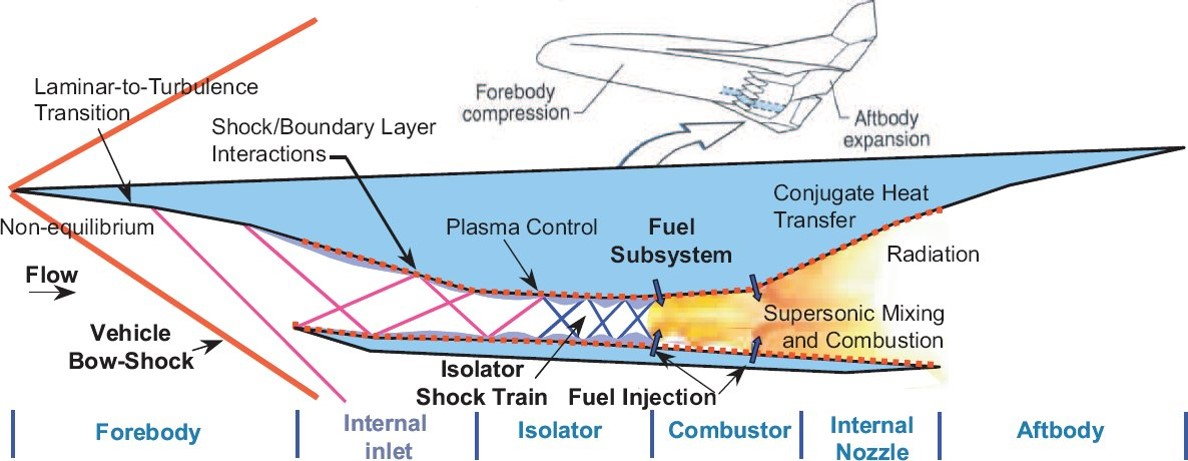
\includegraphics[width=\textwidth]{Figures/scramjet.jpg}
\caption[Scramjet Diagram]{Diagram of a typical scramjet engine, showing shocks produced within the engine. \cite{scramjetFig}}
\label{fig:scramjet}
\end{figure}


\begin{figure}
\centering
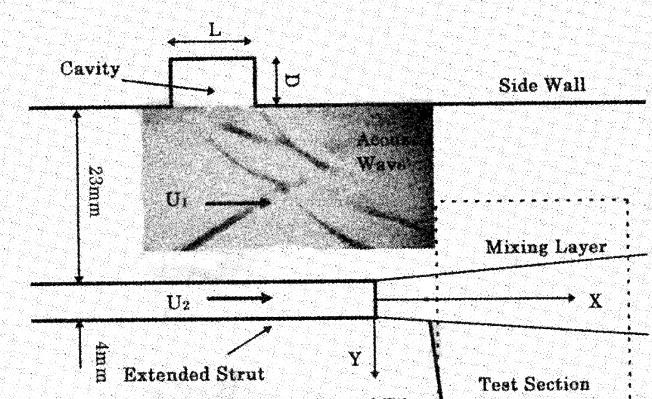
\includegraphics[height=3in]{Figures/CavMix.jpg}
\caption[Cavity-Actuated Mixing]{Mixing enhanced by acoustic waves produced by a side wall-mounted cavity \cite{sato1999advanced}}
\label{fig:sato}
\end{figure}

 
%% Chapter Template

\chapter{Theory} % Main chapter title

\label{Chapter2} % Change X to a consecutive number; for referencing this chapter elsewhere, use \ref{ChapterX}

\lhead{Chapter 2. \emph{Theory}} % Change X to a consecutive number; this is for the header on each page - perhaps a shortened title

%----------------------------------------------------------------------------------------
%	SECTION 1
%----------------------------------------------------------------------------------------

\section{Cavity Flame-holding}
Cavity flame-holding is a well-researched topic in hypersonic combustion \cite{}. 



%----------------------------------------------------------------------------------------
%	SECTION 2
%----------------------------------------------------------------------------------------

\section{Cavity Acoustics}





%------------------------------------------------------------------
%    FIGURES
%-----------------------------------------------------------------
\newpage

\begin{figure}
\centering
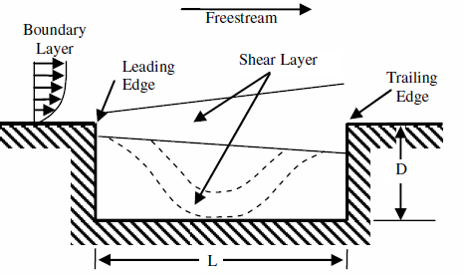
\includegraphics[height=3in]{Figures/CavityDiagram.png}
\caption[Diagram of typical cavity]{Typical hypersonic cavity schematic \cite{lazar2008control}.}
\end{figure}
% Chapter Template

\chapter{Experimental Setup} % Main chapter title

\label{Chapter3} % Change X to a consecutive number; for referencing this chapter elsewhere, use \ref{ChapterX}

\lhead{Chapter 3. \emph{Experimental Setup}} % Change X to a consecutive number; this is for the header on each page - perhaps a shortened title

%----------------------------------------------------------------------------------------
%	SECTION 1
%----------------------------------------------------------------------------------------

\section{Expansion Tube}

The expansion tube is an impulse flow device similar to a shock tube. With an expansion tube, a high pressure gas is used to accelerate a volume of lower pressure gas to certain conditions required for supersonic testing. For the case of supersonic cavities, these conditions need to be similar to those found in the combustor of a scramjet engine. With the expansion tube at Lafayette College, Mach numbers between 2 and 4 have been attained. 

%-----------------------------------
%	SUBSECTION 1
%-----------------------------------
\subsection{Sections}

The expansion tube consists of four sections, which are highlighted in Figure \ref{fig:tubelabeled}. The four sections are: the driver, the double diaphragm, the driven, and the expansion, as listed from upstream to downstream. Initial conditions of the tube set by the operator determine test conditions within test section. These initial conditions include pressure ratios between the sections as well as the gases used in the sections. Each section is divided by plastic diaphragms at the start of each tests. These diaphragms allow the sections to be filled to the different pressures with the different gases required for testing.

The driver section is contained at a high pressure at the start of a test. This section is rated to be filled up to 800 psi. Non-combusting tests performed were run with a driver pressure of 225 psi. With higher pressures, faster test velocities of the test gas can be achieved. 

The double diaphragm serves as a starting mechanism for the experiments. It is filled to an intermediate pressure about half the driver pressure. This section is a very small volume (\textbf{place volume here}), which when vented, creates a large pressure drop across the most upstream diaphragm, causing it to break. The breaking of the diaphragm begins a chain reaction, starting the test. 

Once the test begins, the test gas, which is contained in the driven section at a sub-atmospheric pressure, is accelerated by the driver gas. The test gas travels down the tube, compressed and shock heated until it breaks through the last diaphragm between the driven and expansion sections. This last section differentiates an expansion tube from a shock tube. With the addition of the last diaphragm, the expansion section can be kept at an even lower pressure than the driven section. When the diaphragm between these sections break, the test gas experiences  expansion and unsteady acceleration, allowing faster freestream velocities and higher Mach numbers in the test section. 

%-----------------------------------
%	SUBSECTION 2
%-----------------------------------

\subsection{Diaphragms}
To separate the four sections, plastic diaphragms were placed at the boundary between these sections. These diaphragms were used to keep a pressure differential between the driver, double diaphragm, and driven sections. The pressure differential between these sections was a maximum of 120 psi for non-combusting tests. Another diaphragm was used to separate the test gas in the driver and the expansion gas in the expansion section. Depending on the test conditions, this diaphragm was required to withstand a maximum pressure differential of 1 psi. 

Different thickness diaphragms were required, depending on the pressure differential between the sections. All diaphragms used for the driver and double diaphragm sections were cut from polycarbonate sheet. In order to determine the required diaphragm thickness, calculations were performed, utilizing known material properties and spherical pressure vessel relationships. Since the diaphragm is expected to expand to a near half sphere before breaking, a thin wall spherical pressure vessel relationship was used to determine the maximum pressure the plastic could withstand. This relationship, shown in Equation \ref{eq:spherePV}, was utilized to determine a range of thicknesses of the polycarbonate sheets to be used for different pressure conditions. 

\begin{equation}
\sigma_{uts} = \frac{P~r}{2t}
\label{eq:spherePV}
\end{equation}

After initial testing of these diaphragms, it was determined this relationship provided an overestimation of about 185\% for the breaking pressure of a specific thickness of diaphragm. Since the polycarbonate sheets come in certain stock thicknesses, several thicknesses were purchased and testing was performed to determine the breaking pressure of each diaphragm. For this testing, a 1/4" polycarbonate sheet was placed at the upstream end of the double diaphragm and the thinner test sample was placed at the downstream end of the double diaphragm. The double diaphragm was then filled slowly. When the downstream diaphragm broke, the highest pressure reached was recorded. This procedure was repeated for other thicknesses of diaphragms. The results from these burst tests is shown in Table \ref{Table:Burst}. A majority of the non-combusting tests run were at a driver pressure of 225 psi, so 0.045" diaphragms were selected, as they have a higher burst pressure than the pressure differential between the driven and the double diaphragm, but not higher than the differential between the driver and the driven sections. These diaphragms reliably broke for each test.

\begin{table}
\centering
\begin{tabular}{|c|c|c|}
\hline
\hline
Thickness (inches) & Trial 1 Burst Pressure (psi) & Trial 2 Burst Pressure (psi)\\ 
\hline \hline
0.010 & 32 & n/a \\

0.015 & 60 & n/a \\

0.020 & 93 & 92 \\

0.030 & 123 & 125 \\

0.045 & 153 & 163 \\

1/16 & 233 & 274 \\

3/32 & 341 & n/a \\

\hline \hline

\end{tabular}
\caption[Diaphragm Burst Pressures]{Diaphragm burst pressures at various thicknesses of polycarbonate sheets.}
\label{Table:Burst}
\end{table}

Occasionally, after a test was run, it was noticed that the pieces of the diaphragm completely broke off, sending these pieces down the tube. Having these large pieces of diaphragm sent down the tube is unwanted. These large pieces can cause serious damage to the model in the test section, as well as damage to other parts of the tube. During one test, a large piece of diaphragm struck the nose of the blunted cylinder model, causing severe damage to the pressure transducer located at the nose. It was also observed that pieces of diaphragm nicked the observation windows on the test section. These damages needed to be avoided, so one proposed solution to this problem was to score the diaphragms. A short, shallow incision on the outside of the plastic in an "X" pattern would create failure modes which the diaphragm should break along. These failure modes cause the diaphragm to petal, ideally opening as wide as the tube, with the entire diaphragm intact. 

Burst tests were performed on several scored diaphragms of 0.045" thickness.  This scoring was performed by hand with a knife, applying light pressure. The resulting score appeared as deep scratches in an "X" pattern. The results of the tests showed no significant decrease in burst pressure. In fact, all of the tests showed a higher burst pressure for the scored diaphragms than for the not scored ones. This could be due to the scoring allowing the plastic to deform further before bursting. It could also be due to the plastic being from a different batch sheet than the plastic used for earlier burst tests. Regardless of the reason, the results showed that the scored diaphragms could still be used. It was also found that good petalling of the diaphragm occurred, with minimal, if any, loss of diaphragm pieces down the tube. Because of these results, scoring of the diaphragms has become a regular step in the setup of the tube for each test.  




%----------------------------------------------------------------------------------------
%	SECTION 2
%----------------------------------------------------------------------------------------

\section{Models}

For testing, a cavity model was designed and manufactured. The designed cavity, as shown in Figure \ref{fig:cavModel}, was designed to be mounted with the current mounting system in the test section. This mounting system consists of a rectangular upright with thru holes for shoulder bolts. The three holes seen in Figure \ref{fig:cavModel} are in line with the existing holes in the mounting system. This allows one to swap out models in the test section quickly in between tests. 


%-----------------------------------
%	SUBSECTION 1
%-----------------------------------
\subsection{Design Choices}

While designing the cavity, several choices had to be made about the geometry of the model as well as the features of the cavity. Brass was chosen as the material due to its relatively low cost as well as its ability to be easily machined. Brass also holds up well to the conditions experienced in the test section during testing. 

The overall size of the brass was chosen based on the size of the core flow, the flow volume where the desired freestream conditions exist, exiting the tube into the test section as well as the requirement to be affixed to the existing mounting system. The size of the core flow coming out of the tube begins about the diameter of the tube itself. However, it grows smaller as the length from the tube exit increases. It is important that the area of interest (the cavity) is contained entirely within this core flow. Knowing the cavity would sit a few inches from exit of the tube, a width of 2.5 inches was chosen for the brass. This would ensure that the core flow, at the time it interacts with the cavity, would entirely encapsulate the cavity. A total height of 1 inch was chosen because it allowed the rectangular hole for the mounting system to be machined to the correct depth that aligned the thru holes for the shoulder bolts. It was designed that after the rectangular hole was made in the brass, a thickness of 1/4 inch was left. This was chosen because the cavity exists relatively close to the mounting system and at least 1/8 inch of material needed to be left between the top of the mounting system and the bottom of the cavity to ensure the part could be machined without any issues. 

The cavity itself was placed \textbf{THIS FAR AWAY FROM THE FRONT} in order to develop the flow over the flat plate. Flow conditions experienced by the cavity should match closely to flow conditions experienced in scramjet engines, including boundary layer conditions. The thickness of the boundary layer was estimated to be on the order of \textbf{Blank} for the length chosen. This estimation was made using the relationship shown in Equation \ref{eq:BL}, where Re is shown by the relationship in Equation \ref{eq:Re} and x is the distance to the front of the cavity from the leading edge of the model. For consistency with other researchers and their boundary layer thickness, as length of \textbf{THIS LENGTH} was chosen.

\begin{equation}
\delta = \frac{0.37x}{(Re_x)^{1/5}}
\label{eq:BL}
\end{equation}

\begin{equation}
Re_x = \frac{\rho U_\infty x}{\mu}
\label{eq:Re}
\end{equation}

At the upstream end of the cavity model, there exists a wedge. Flow over a flat plate leading up to the cavity was desired. The wedge was designed in order to redirect any shock waves away from the cavity. These shock waves have the ability to adversely affect test results if they interact with the cavity. Calculating shock wave angles for several wedge angles and calculating where the shocks would reflect off the walls of the test section, a wedge angle of \textbf{WEDGE ANGLE HERE} was chosen. This angle created a shock of \textbf{SHOCK ANGLE HERE}, which, when reflected through the shear layers surrounding the expansion tube core flow, did not reflect into the cavity.

The stability of the model was also an important design consideration. With the flow conditions experienced in the test section, a stagnation pressure of nearly 1,000 psi could be experienced by the model. With the model's front wedge shape, a net force in the vertical direction of nearly \textbf{Force Here}, coupled with a relatively large moment arm has the potential to result in some movement from the cavity. To ensure the bending was as minimal as possible, a triangular brace was manufactured to secure the base of the cavity to the test model stand. This reduced the effective moment arm to provide structural support and stability to the model. This triangular support is pictured in the test section assembly in Figure \ref{fig:cavTestSection}.


%-----------------------------------
%	SUBSECTION 2
%-----------------------------------
\subsection{Modular Design}

Because the acoustic properties are the main focus of this thesis, it was important to design a model in which these acoustic properties could change. Frequency is one main acoustic property that was chosen to be varied with these cavities. Using Heller and Delfs relationship, Equation \ref{eq:freq}, varying the length of the cavity would lead to different cavity frequencies \cite{heller1996letter}. However, the L/D is also an important parameter in the flame-holding characteristics of these cavities. This ratio determines the recirculation properties as well as residence time within the cavity. A modular design was then chosen so that a range of L/D ratios could be tested. For good flame-holding characteristics, a L/D between 4 and 10 has been shown to provide those characteristics \cite{ben2001cavity}. For the design, having a constant depth would result in a change in length of the cavity with a change in L/D ratio. Thus, as the L/D ratio changes, so do the flame holding properties as well as the dominant frequencies within these cavities. 

For the modular design, a 1/8-inch deep, 1 5/8-inch long cavity was created, as shown in Figure \ref{fig:cavModel}. Along with the large cavity, different sized inserts were manufactured. The length of the cavity was chosen so that these inserts could be attached, decreasing the overall length of the cavity, and achieving the desired L/D. Six inserts were manufactured to create L/Ds of 5, 7, and 9, each with two varients of a downstream wall. These inserts are shown relative to the base cavity in Figure \ref{fig:cavInserts}. At each L/D, there was one insert with a flat wall and one insert manufactured with a 30$^\circ$ incline. This angled incline, as shown by Ben-Yakar \cite{ben2001cavity}, has the ability to suppress the acoustic waves while still retaining flame holding characteristics. The angled wall does not allow the pressure waves to propagate within the cavity space. This allowed for the comparison of flame-holding abilities of the cavity with and without strong acoustic waves present at each L/D. This modular design gave a relatively wide spectrum of cavity conditions to test with a relatively easy means of changing these conditions for each test. 

%-----------------------------------
%	SUBSECTION 3
%-----------------------------------
\subsection{Implementation}

For each test, it was determined which L/D needed to be tested. After this choice was made, the corresponding insert was installed and the test section mount was prepared for the cavity model to be placed in it. Depending on which model was mounted in the test section before the cavity test, the mounting stand may have needed to be adjusted.  Since the area of interest is the cavity, it was placed at the center of the viewing window for the schlieren to focus directly on it. Once the test mount was correctly positioned, the cavity model was attached to it with three shoulder bolts. The triangle support was then attached between the model and test stand, providing extra stability when the test runs. Once the model is mounted, switching between L/D inserts is as easy as removing the test section door and three screws holding the cavity insert to the model. A photo of the cavity installed in the test section is shown in Figure \ref{fig:cavTestSection}.


%----------------------------------------------------------------------------------------
%	SECTION 3
%----------------------------------------------------------------------------------------

\section{High Speed Pressure Transducers}

Placed along the tube at various locations are piezoelectric pressure transducers. These pressure transducers provide both analog and digital data for each test run. The analog data allows for the observation of shock strength and the digital data allows for the calculation of shock velocity. When the shock passes by one of these sensors, it registers as a very sharp increase in pressure. Knowing the time at which these shocks arrive at the various transducer locations, along with the location of the transducers relative to each other allows for the shock speed calculation. 

Ideally, calculating the time step between the arrival of each shock could be done by observing the time between the sharp spike in the analog pressure signal. However, to achieve a more accurate calculation of the time, a digital National Instruments card with a maximum sampling frequency of 20 MHz was used. The faster sampling frequency allows the small time step to be calculated far more accurately than the analog National Instruments card used for the analog pressure signals. 

In order to produce the digital signal required for the LabVIEW timer counter program to calculate the time between signals, a simple analog to digital circuit was designed. The design of the circuit was based off of previous work done by Helen Hutches \cite{Hutchens2015}. This circuit, as shown in Figure \ref{fig:timercircuit}, produces a 5V signal when an analog voltage is higher than a certain threshold. This threshold reference voltage is determined by three potentiometers connected to the circuit. The three potentiometers allow three different reference voltages to be set for up to six pressure transducer signals. When the analog voltage is lower than this reference voltage, the output of the circuit is 0V. This allows the digital data acquisition card to read either a HIGH (5V) signal or a LOW (0V) signal and interpret that as a digital signal. 

This digital signal is also used to trigger the camera to record. The LabVIEW program, once getting a signal from a specified pressure transducer will generate a 5V TTL pulse. 

%-------------------------------------------------------------
%	 SUBSECTION 1
%-----------------------------------------------------------

\subsection{Circuit}
The circuit operates using three op-amps and one pull up resistor. The op-amps, as shown in the center of Figure \ref{fig:timercircuit}, read the signal from the potentiometers. The voltage level, between 0 and 5 volts, from the potentiometer is set by the user. The op-amp compares this voltage to the voltage signal received through the BNC connectors. These BNC connectors are the analog voltage from the pressure transducers along the tube. If the voltage coming from the pressure transducers is below the voltage set by the user, the output of the circuit is 0V or a LOW digital signal. If the voltage is above this set voltage, the output of the circuit is 5V or a HIGH digital signal. 

The purpose of this circuit is to convert the analog signal sent by the pressure transducers into a digital pulse that can be read by the digital card. The potentiometers are put in place so the digital pulse is only sent when the shock wave passes by the transducer, rather than noise actuating the digital signal to be sent. Reliable results have been achieved with this circuit, but there are some cases in which this system has failed, but in the next section, it will be explained how to fix some of the more common problems and check for specific errors.


%----------------------------------------------------------
%	 SUBSECTION 2
%---------------------------------------------------------

\subsection{Implementation and Troubleshooting}

When using the timer counter box, make sure the box is plugged into the power supply. Once the box has power, turn on the power supply associated with the inverting circuit. Once these are powered, the blue amplifier boxes should be turned on to supply power to the transducers. Set the appropriate gains on these boxes. The appropriate gains are based on what magnitude signal is desired. The LabVIEW program will only read signals between 0 and 5V. The pressure transducers output 0-5V for a pressure range of 0 to 100 psi. However, the pressure these transducers will be exposed to are only between 10 and 20 psi, resulting in a 0.5 to 1V signal. Setting the gain to 5 allows that signal to be amplified to to between 2.5 and 5V. Having a larger signal allows for the comparator circuit to operate more easily. One can set the comparator nominal voltage with confidence, as the larger signal allows for a larger margin of error on the set comparator voltage. This gives more confidence that the signal coming into the comparator circuit will be large enough to trigger a digital signal. 

Once the physical systems are powered and ready, run the two LabVIEW programs for the capturing of the digital signals as well as the analog signals. The analog program filename is ''BasicHighSpeedOscillosope-fixed.vi'' and the digital program filename is ''CountersWorking.vi'' For the analog signal, an input is required for sampling rate and time to take data. The typical sampling rate and time for tests is 1MHz and 10,000 $\mu$s. The digital program asks for a user input of ''milliseconds to wait.'' This is the amount of time the program should wait until sending the 5V TTL pulse to the camera. Typically, this value is set to 0. 

One common problem with this circuit is that no digital signal is sent from the circuit itself. To check for this, use a function generator and an oscilloscope. Hook up the oscilloscope to one of the digital out wires of the box as well as the output of the function generator. Table \ref{Table:pins} shows the number of the digital out wire to its corresponding number. Attach the function generator to the corresponding BNC connector. A T-connector is needed to split the output signal from the function generator. Send a 5V amplitude sine wave from the function generator. The corresponding signal from the box should be a square wave. If there is no square wave present, check that the potentiometer is not too high or too low. The square wave should get wider or narrower depending on the position of the potentiometer. If there is still no signal coming from the box, there may be a burnt out op-amp. If, however, there is no signal coming from any of the outputs, it is unlikely all of the op-amps burned out. In this case, there may be a wiring issue. For this, check continuity between the signal coming in and the signal coming out to make sure voltages at each connection are what they are supposed to be. Some alteration of the circuit may be required in this case. However, that is unlikely, and the problem is likely to be that the potentiometer level was set too high.




%---------------------------------------------------------
%    SECTION 4
%-----------------------------------------------------------------------------------

\section{Infrared Sensor}

Test time is important for the correlation of schlieren image data. Because the two systems are initiated simultaneously, the IR data corresponds easily to the image data. Knowing when the test gas reaches the model and for how long the test gas is flowing over the model allows for the extraction of frames that equate to just the test time. Although it is possible by inspection to see when the test gas arrives at the model, it is not always obvious or as accurate. The arrival of the test gas produces shock waves at a different angle than the helium behind the incident shock wave, but this change in angle might not be very large, depending on the change in velocity. However, with the IR data, it can be closely estimated when the test gas should reach the model and for how long the model experiences the test gas. 

Test time can be estimated using an X-T diagram. A sample X-T diagram is shown in Figure \ref{fig:XT}. This diagram is generated using compressible flow equations under an inviscid assumption. The lines represent important flow characteristics, including shock wave or expansion fan locations. The x-axis represents the spatial location along the tube, while the y-axis represents time. The time between the second and third line at the test section location represents the time which the test gas passes by the test section at the proper conditions. This ideal test time can be used to estimate the experimental test time, but a more accurate measurement of test time using the IR sensor is needed for proper image correlation and analysis.

The sensor used with the expansion tube at Lafayette is a Judson J10D series Indium Antemonide (InSb) sensor. These detectors have photovoltaic sensors that produce a current when exposed to infrared radiation. The sensor has the ability to be utilized for both absorption as well as emission sensing techniques. These techniques are explained in detail in a subsequent subsection.

%------------------------
%    SUBSECTION 1
%------------------------

\subsection{Design of System}
The alignment and placement of the various components is important for the proper collection of the IR light from the tube. The setup, as depicted in the diagram in Figure \ref{fig:IRschematic}, includes a slit, a concave mirror, and a flat mirror. The slits affect the spacial resolution of the incoming signal. If the slits are too wide, the sensor captures some of the scattered light, which shows up as a gradual increase in signal. If the slits are too narrow, not enough light can be captured by the sensor to show a good signal. The slit width is still being fine-tuned for the system in place, but the typical width for the slits is between 1 and 3 mm \cite{flower1976experimental}. 

The sensor itself has a circular pickup area of about 2mm in diameter. Because of this, the IR light from the tube needs to be focused. Once the light passes through the slits, it reflects off of a concave mirror. This concave mirror, with a focal length of \textbf{insert focal length}, focuses the light to a small point, just about the size of the sensor. The flat mirror is used to collapse the system so it can fit in a relatively small area. The entire system is contained in a box, as shown in Figure \ref{fig:IRlabel}. Both mirrors are gold coated, as gold is very efficient at reflecting IR light. Since most of the testing is done during the day, a box was constructed to block out any ambient light from the room. The system is attached to the support structure of the tube by a 1/2" aluminum plate cantilever. Some bending, less than 1/16",  is present at the end of the beam where the setup is supported, but it is not enough to affect the collection by the IR system. 

%------------------------
%	 SUBSECTION 2
%------------------------

\subsection{Set Up}


To achieve the sensitivity required for the sensor, the operating temperature of the IR detector is about 77K, and the detector must be cooled with liquid nitrogen. Using the funnel to avoid spillage of the liquid nitrogen onto the cable connections or viewing window of the sensor, a few hundred milliliters were poured into the hole at the top of the sensor. When the sensor reaches the correct temperature, an eruption of cool gas occurs. It is important to wait until this eruption completes because the buildup of gas can cause the cap to blow off. Once the eruption subsides, the cap can be replaced to the top of the sensor and power can be supplied to the amplifier. 

After power is supplied to the sensor through the amplifier, it is important to check that the system is aligned. Since the setup is attached to the support structure and not the tube itself, the recoil of the tube or the moving of the tube to replace diaphragms can alter the alignment of the window to the focusing mirror. To re-align the system, a stainless steel LED tube was constructed. This tube fits within the porthole on the back side of the tube, aligned with the port for the IR sensor. With the LED on and lined up with the inside wall of the far side of the tube, check the light source path. Be sure that the thin slit of red light hits the small sensor area. Adjust the flat mirror as needed to align the slit of red light with the IR sensor pickup area. Once the system is aligned, remove the LED tube and replace the plug in that port. The system at this point is aligned and ready for a test.  

%------------------------
%     SUBSECTION 3
%------------------------

\subsection{Absorption}

One method of data capturing that can be used is infrared absorption. The absorption method is based on the principle that different gases absorb radiation at different amounts. For absorption tests, an infrared light is placed behind a sapphire window on the other side of the tube. This IR light source provides the sensor with a baseline IR emission reading. As different gases pass by the sensor, they absorb some of the IR light, resulting in a different level of IR signal at the sensor. Measuring the time at the absorption level that corresponds to the test gas corresponds to the test time within the test section. Although the sensor is capable of reading the IR signal with this method, the emission method has provided more reliable measurements of test time. The emission method only allows for signal to come to the sensor when the hot test gas is passing by, whereas the absorption method also shows when the other gases pass by the sensor. A typical voltage trace of the absorption method is shown in Figure \ref{fig:IRabsorption}. It is clear that there is much uncertainty of which test gases are passing by the IR sensor during this pressure trace. There are no sharp spikes in signal, but rather, the signal exhibits low sloped voltage changes. Also, at the end of the test, the IR signal should return to its baseline. However, the signal continues to rise, and even experiences a hump near the end of the test. This uncertainty in the voltage trace made it difficult to experimentally measure test times. Because of this, the emission method has been used primarily in the non-combusting tests and will continue to be used in the combustion tests. Further testing and tuning of the system would be required to capture more meaningful information with this absorption method. 


%------------------------
%     SUBSECTION 4
%------------------------

\subsection{Emission}

As gases are heated, they emit IR radiation at different wavelengths. Using a filter, other wavelengths that are not these specific wavelengths, will not pass to the detector. For the non-reacting flows, a 5\% CO$_2$ in nitrogen mixture emits IR within a 180nm bandwidth centered at 4.248$\mu$m. Placing the filter in front of the sensor allows the sensor to detect when, and for how long, the test gas, CO$_2$ passes by the sensor. Knowing how long the gas passes by the sensor allows for a direct measurement of test time in the test section. Due to the sensor's close proximity to the test section, the test time extracted from the IR data is very close to the test time for the models in the test section. An example of the voltage trace produced by the sensor using the emission method is shown in Figure \ref{fig:IRemission}. 

Shown in the image are a few artifacts known about this system. Included in this voltage trace is the voltage of the pressure transducer at the same location as the IR sensor for reference. The sharp peak of the pressure signal indicates the arrival of the initial shock wave. This indicates that helium is flowing by at that time. However, there is also an increase in the IR signal. The current hypothesis is that this signal is the presence of light produced by burning diaphragm particles flying down the tube. The next spike, however, is the $CO_2$ passing by the IR source. Measuring the length of time this spike occurs over leads to the estimation of experimental test time. 

It is also noted that the voltage trace does not exhibit sharp spikes in signal. This is due to the size of the slit width, which was too open for this test. This slit width allowed forward-scattered light to be picked up by the sensor. It was assumed that the true start of the signal is halfway up the slope. However, it is important to continue fine-tuning the system and the slit width in order to eliminate this uncertainty.

%-------------------------
%      SUBSECTION 5
%-------------------------
\subsection{Premature Ignition}

The IR sensor will also be used to determine if pre-combustion occurred during a test. It is expected that if the reaction combusts upstream of the test section, it will result in a very large spike in IR signal. This will indicate that combustion did not originate at the cavity, but rather upstream of the cavity. Since the combustion tests are being used to test the flame-holding characteristics of the cavity, it is imperative that ignition originates at the cavity. 


%---------------------------------------------------------
%    SECTION 5
%-----------------------------------------------------------------------------------

\section{Schlieren Imaging}

The images captured for the tests were done so using a high speed camera with a z-type schlieren system. A diagram of the schlieren system at Lafayette can be seen in Figure \ref{fig:schlieren}. The camera used for image capturing is a Phantom Miro m310 camera, capable of taking images up to 250,000 fps. However, as the recording frame rate increases, the resolution of each image decreases. For testing, a nominal frame rate of 77,000 Hz was used, as this provided a sufficient frame rate without sacrificing too much resolution. The resolution at which the images were taken at in this study is \textbf{Frame Rate Here}. A sufficient frame rate in this context is one in which one test is captured within 500-1,000 frames. Also, to observe the frequencies within the cavity, the frame rate must be several times higher than the expected frequency of the acoustic waves. With L/D of 5, 7, and 9 having expected frequencies of 30 kHz, 21.4 kHz, and 16.7 kHz, respectively, a frame rate of 77 kHz would provide between 3 and 5 frames to observe the propagation of the waves.

The schlieren effect operates on the principle that light refracts in air due to changes in density. This can be observed firsthand on a hot day. The rippling effect one can see above a road on a hot day is the light refracting due to the different densities of the air, caused by differences in local air temperature. Schlieren imaging takes advantage of this principle by placing a knife edge at the focal point of the system. As light is refracted due to a change in density, this light gets blocked out by the knife edge, showing up as a dark spot in the captured image. Light that is not refracted continues through to the camera unblocked. 

This type of imaging is important to see the various shock waves produced during testing. Since shock waves produce very sharp density gradients, a system that is capable of capturing these density gradients at high speeds is very useful. Typical test time of the non-reacting tests, the time in which the model experienced the test gas,  was on the order of about 300 microseconds. With this camera, nearly 23 images were captured for the test time.  With this many frames, it was possible to time correlate the images as well as extract dominant frequencies within the cavities.

Further information about the system, including more detail on how the system works and how to calibrate and align the system at Lafayette can be found in Ray Sanzi's honors thesis \cite{Sanzi2016}.



%-------------------------------------------------------------------
%    FIGURES
%------------------------------------------------------------
\newpage

\begin{sidewaysfigure}
\centering
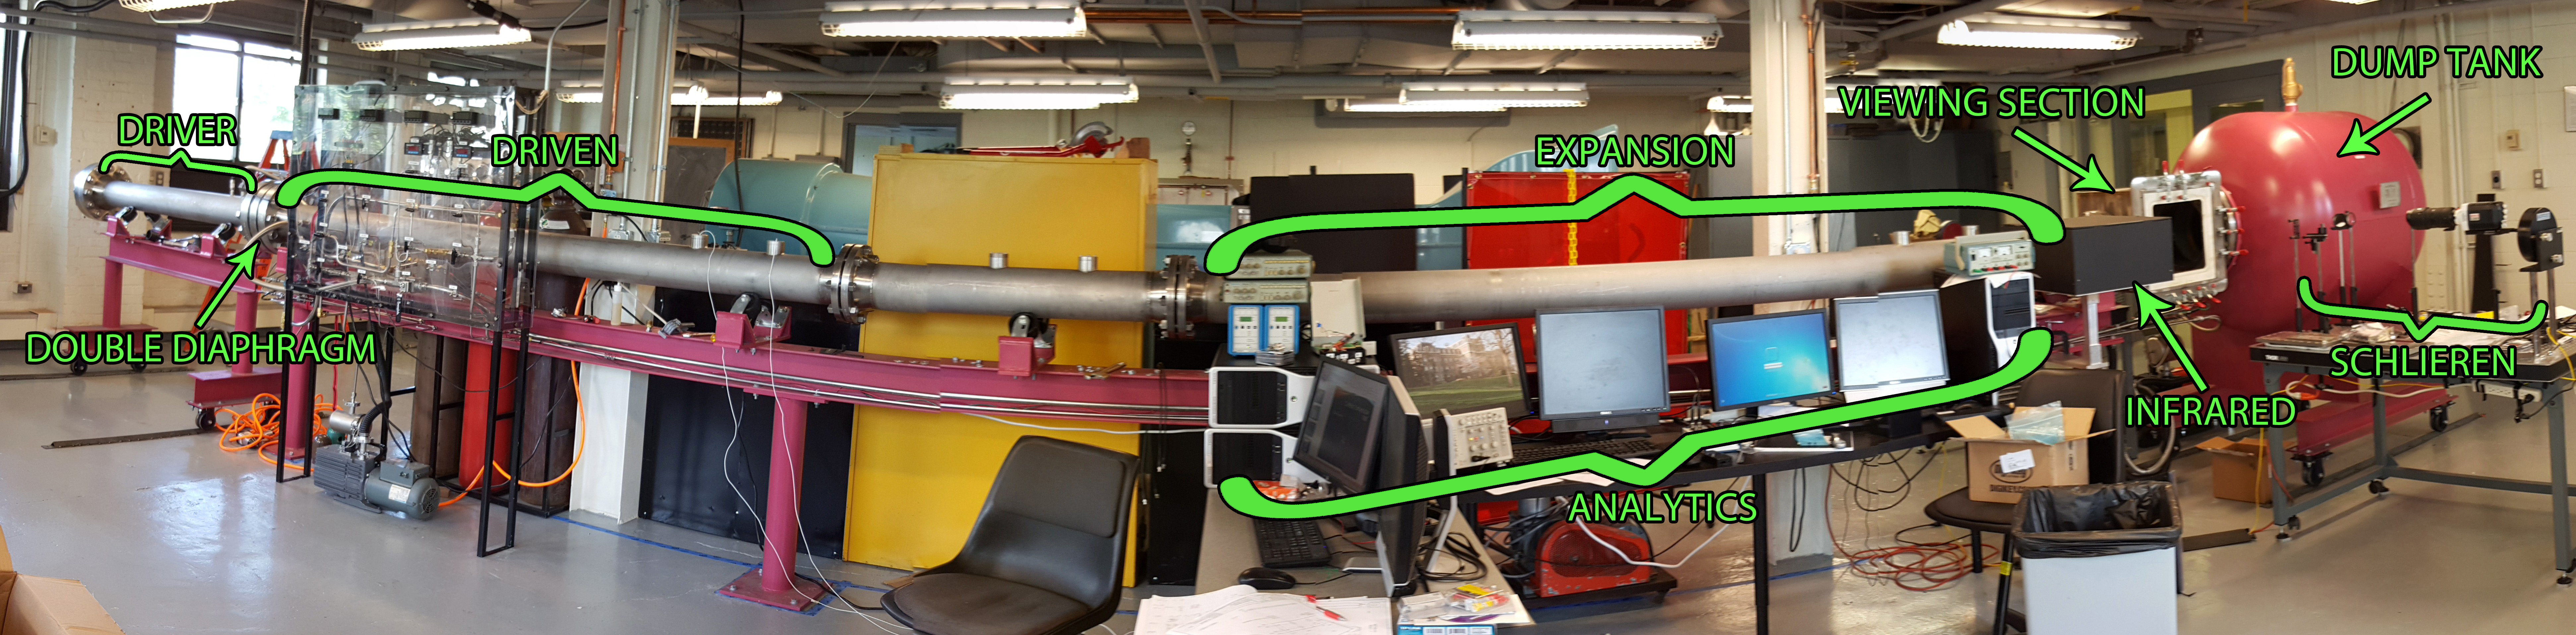
\includegraphics[width=\textwidth]{Figures/TubeLabeled.jpg}
\caption[Annotated Expansion Tube]{Annotated photograph of the expansion tube at Lafayette College}
\label{fig:tubelabeled}
\end{sidewaysfigure}

\begin{figure}
\centering
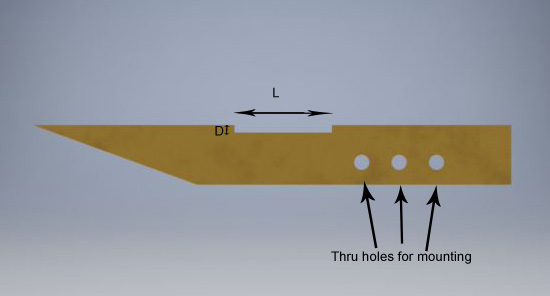
\includegraphics[height = 3in]{Figures/Cavitylabel.jpg}
\caption[Cavity 3D Model]{3D rendering of cavity used in testing}
\label{fig:cavModel}
\end{figure}

\begin{figure}
\centering
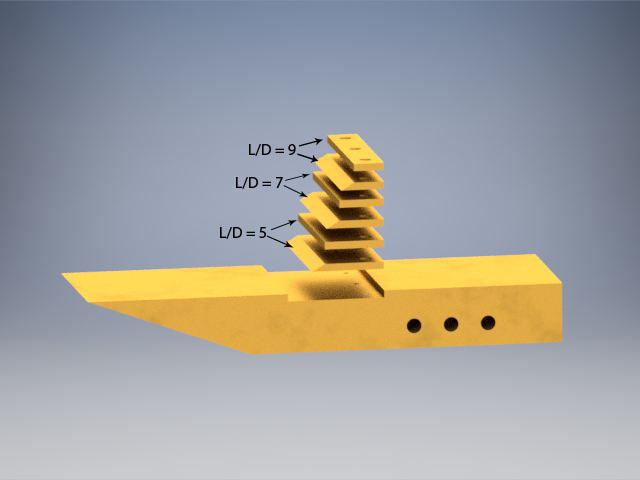
\includegraphics[height = 3in]{Figures/CavityInserts.jpg}
\caption[Cavity Model with Inserts]{3D rendering of cavity with various inserts to alter L/D}
\label{fig:cavInserts}
\end{figure}

\begin{figure}
\centering
\includegraphics[width=\textwidth]{Figures/Circuit.png}
\caption[Circuit Diagram for Timer Counter Box]{Circuit diagram for timer counter box}
\label{fig:timercircuit}
\end{figure}


\begin{figure}[p!]
\centering
\includegraphics[width=\textwidth]{Figures/DataFlow.png}
\caption[Data Flow for High Speed Pressure Transducers]{Data flow for high speed pressure transducers}
\label{fig:DataFlow}
\end{figure}
\clearpage

\begin{figure}
\centering
\includegraphics[height = 3in]{Figures/IRschematic.png}
\caption[IR setup diagram]{Schematic of the IR setup for the expansion tube.}
\label{fig:IRschematic}
\end{figure}

\begin{figure}
\centering
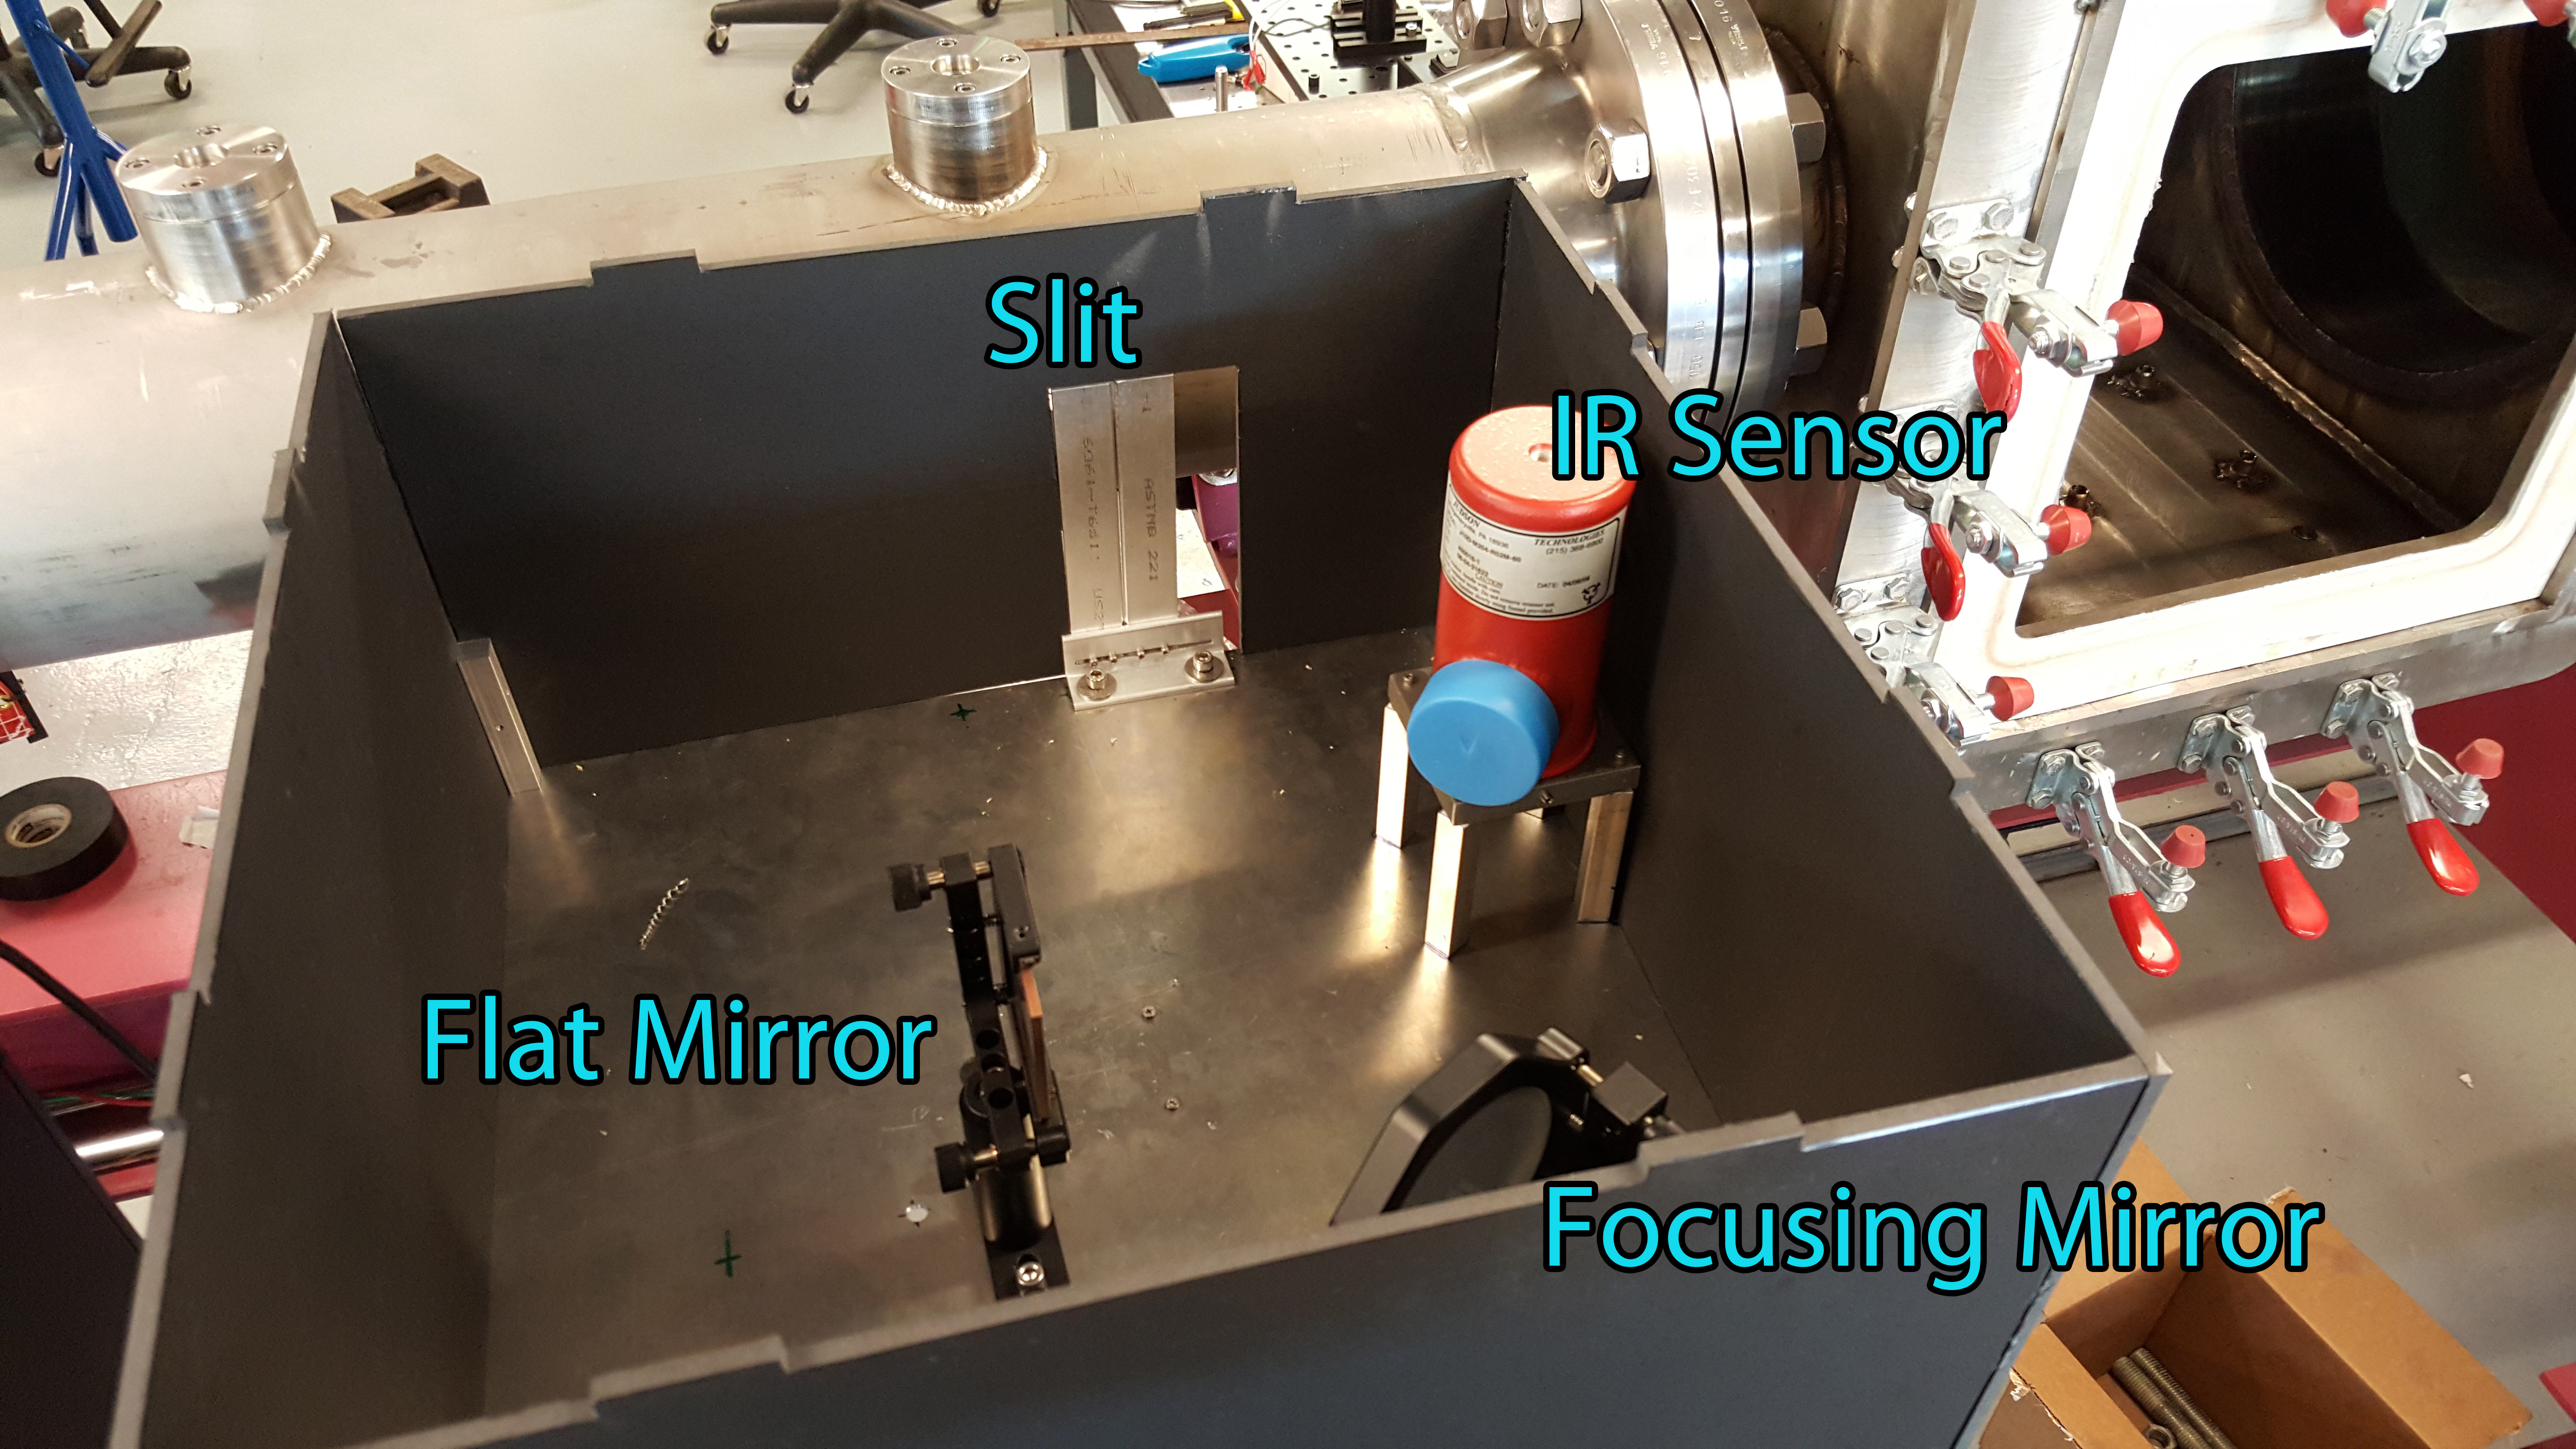
\includegraphics[height = 3in]{Figures/IRLabeled.jpg}
\caption[Labeled photograph of IR setup]{Photograph of actual IR setup in the lab.}
\label{fig:IRlabel}
\end{figure}

\begin{figure}
\centering
\includegraphics[height = 3in]{Figures/absorption.jpg}
\caption[Typical IR data utilizing absorption method]{Typical IR data utilizing absorption method}
\label{fig:IRabsorption}
\end{figure}

\begin{figure}
\centering
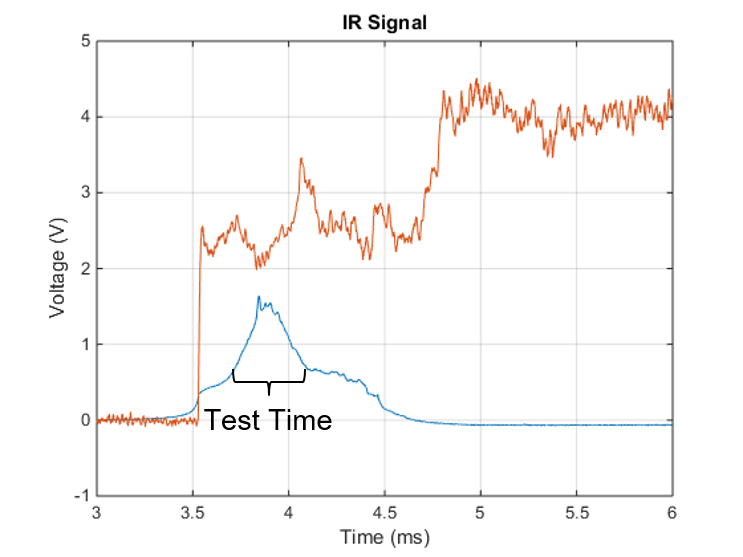
\includegraphics[height = 3in]{Figures/IREmission.png}
\caption[Typical IR data utilizing emission method]{Typical IR data utilizing emission method}
\label{fig:IRemission}
\end{figure}

\begin{figure}
\centering
\includegraphics[width=\textwidth]{Figures/Schlieren.png}
\caption[Schlieren Diagram]{Diagram of schlieren system at Lafayette}
\label{fig:schlieren}
\end{figure} 
%% Chapter Template

\chapter{Experimentation} % Main chapter title

\label{Chapter4} % Change X to a consecutive number; for referencing this chapter elsewhere, use \ref{ChapterX}

\lhead{Chapter 4. \emph{Experimentation}} % Change X to a consecutive number; this is for the header on each page - perhaps a shortened title

%----------------------------------------------------------------------------------------
%	SECTION 1
%----------------------------------------------------------------------------------------

\section{Phase 1}


%-----------------------------------
%	SUBSECTION 1
%-----------------------------------
\subsection{Setup and Conditions}



%%-----------------------------------
%%	SUBSECTION 2
%%-----------------------------------
%
%\subsection{Subsection 2}


%----------------------------------------------------------------------------------------
%	SECTION 2
%----------------------------------------------------------------------------------------

\section{Phase 2}


%-----------------------------------
%	SUBSECTION 1
%-----------------------------------
\subsection{Setup and Conditions}



%-----------------------------------------------------------------
%   FIGURES
%-----------------------------------------------------------------

\newpage
 
%% Chapter Template

\chapter{Experimental Results} % Main chapter title

\label{Chapter4} % Change X to a consecutive number; for referencing this chapter elsewhere, use \ref{ChapterX}

\lhead{Chapter 4. \emph{Experimental Results}} % Change X to a consecutive number; this is for the header on each page - perhaps a shortened title

%----------------------------------------------------------------------------------------
%	SECTION 1
%----------------------------------------------------------------------------------------

\section{Non-Combusting Tests}

In order to directly compare data between the different L/D ratios tested, it was important to keep the conditions nearly the same for all tests. For all non-combusting tests performed, the driver gas was helium at an initial pressure of 225 psi. The test gas was nitrogen at 0.5 psi and the expansion gas was helium at an initial pressure of 0.25 psi. This produced the freestream conditions as follows: M$_\infty$ = 2.32, U$_\infty$ = 2150 m/s, and T$_\infty$ of 411K. 

%-----------------------------------
%	SUBSECTION 2
%-----------------------------------
\subsection{Schlieren}

For each L/D, schlieren images were captured. Figures \ref{fig:5}, \ref{fig:7}, and \ref{fig:9} show the effects the L/D ratio has on mixing abilities. It can be observed that all of these cavities exhibit mixing and show signs of strong acoustic signals. The images captured for an L/D ratio of 5, however, show more disturbances, relatively, within the cavity itself. It is difficult to say with the images, though, how much more mixing exists within the cavity. Further sharpening of the images

Figure \ref{fig:5-30} shows the cavity with an angled downstream wall. With this image, it is very clear that there are little or no acoustic waves present. This is strong evidence in support of the angled wall's ability to suppress the oscillation acoustic waves. However, with the acoustic waves not present, it may be possible that the mixing within the cavity suffers as a result. This will be investigated with the combustion tests in further studies. 

Also captured by the schlieren imaging system is an indication of residence time within these cavities. Dust particles within the test section were dispersed in the flow and some of these particles were drawn into the cavity. Measuring how long these particles take to make one revolution within the cavity can provide an estimate of residence time. Figure \ref{fig:ResTime} shows one such particle traveling over several images. The particle took 68 frames to make one revolution, corresponding to an estimated residence time of about 850 $\mu$s. This corresponds well with the 1ms magnitude residence time achieved by Ben-Yakar \cite{ben2001cavity}.

%-----------------------------------
%    SUBSECTION 3
%-----------------------------------

\subsection{IR}

For some of these tests, IR emission data was captured to measure test time. The test times extracted from the IR data are displayed in Table \ref{Table:IRtest}. Of the test times which include nitrogen, they all correspond well to each other, which implies that conditions were reasonably the same for all tests.  The theoretical test time, which was extracted from an X-T diagram, as shown in Figure \ref{fig:XT}, was about 559 $\mu$s for these tests. However, the compressible flow equations used in generating these X-T diagrams assume the flow to be inviscid. Due to viscous effects that are present in the tube along with non-ideal diaphragm breakage, the experimental test time achieved will be less than the theoretical test time, which is consistent with the data. It is important to note that even the tests without the CO$_2$ signal, the signal being picked up by the IR sensor was indicative of test time, as the test times extracted from these traces are consistent with the test times extracted from the traces with the CO$_2$ mixed with nitrogen. The signal captured from the nitrogen tests is presumed to be hot diaphragm particles flowing with the test gas from the upstream diaphragms.

\begin{table}[]
\centering
\caption[Test time calculated with IR signal]{Test time from IR signal for various test gases. P4 = 225psi, P1 = 0.5 psi, P$_e$ = 0.25 psi.}
\label{Table:IRtest}
\begin{tabular}{c|c|l}

Test Number & Test Time ($\mu$s) & Test Gas\\ \hline
046         & 399        &Nitrogen     \\ 
048         & 443        &Nitrogen     \\ 
049         & 441        &Nitrogen     \\ 
050         & 424        &Nitrogen     \\ 
055			& 429		 &Nitrogen + CO$_2$	\\
056			& 434		 &Nitrogen + CO$_2$  \\
057			& 561 		 &2H$_2$ + O$_2$ + 8N$_2$			   \\
058			& 333		 &2H$_2$ + O$_2$ + 8N$_2$ followed by Nitrogen + CO$_2$			   \\
\end{tabular}
\end{table}

Each test produced an IR trace similar to the one shown in Figure\ref{fig:IRTrace}. As can be seen in this trace, the slit width was too wide for the test, so the IR sensor captured some light scattered forward, as indicated by the sloped increase in voltage signal. The test gas is indicated by the highest level of the signal. Test time is taken to be the time between points on the outside of the nearly flat level of signal. With this method, a consistent measure of test time can be achieved regardless of the amount of forward scattering of light. At this highest level, it is certain that there is is only test gas passing by the sensor. With this method, the estimates of test time are conservative, but consistent. For further information on each IR test, please refer to the table in Appendix \ref{Appendix 3}.


%----------------------------------------------------------------------------------------
%	FIGURES
%----------------------------------------------------------------------------------------
\newpage

\begin{figure}
\centering
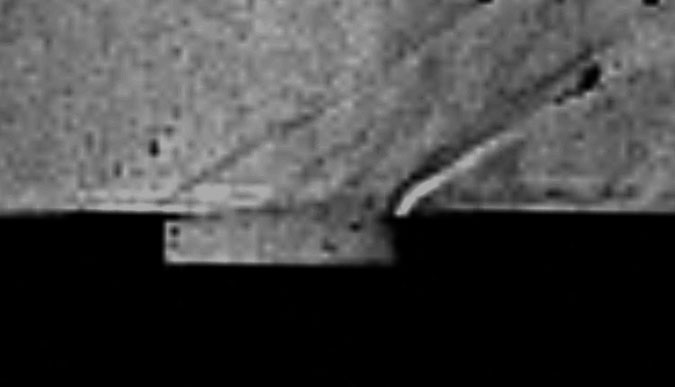
\includegraphics[width = \textwidth]{Figures/5.jpg}
\caption[Schlieren image of cavity. L/D = 5.]{Schlieren image of cavity. L/D = 5.}
\label{fig:5}
\end{figure}

\begin{figure}
\centering
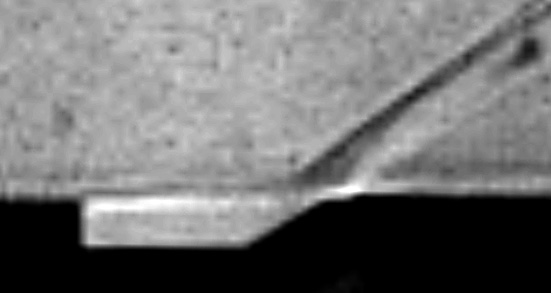
\includegraphics[width = \textwidth]{Figures/5-30.jpg}
\caption[Schlieren image of cavity with angled downstream wall. L/D = 5.]{Schlieren image of cavity. L/D = 5. Downstream wall angle = 30$^\circ$}
\label{fig:5-30}
\end{figure}

\begin{figure}
\centering
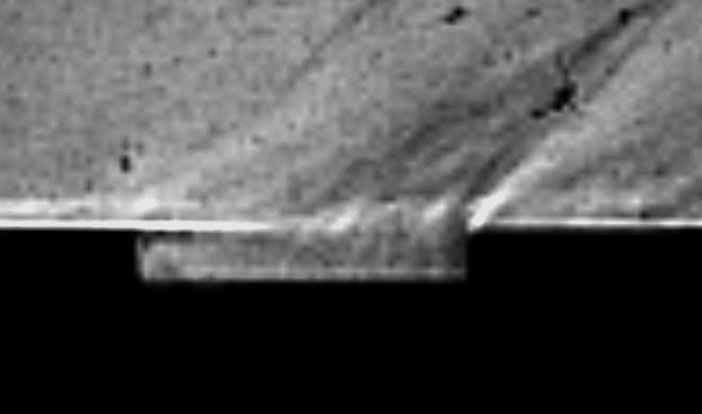
\includegraphics[width = \textwidth]{Figures/7.jpg}
\caption[Schlieren image of cavity. L/D = 7.]{Schlieren image of cavity. L/D = 7.}
\label{fig:7}
\end{figure}

\begin{figure}
\centering
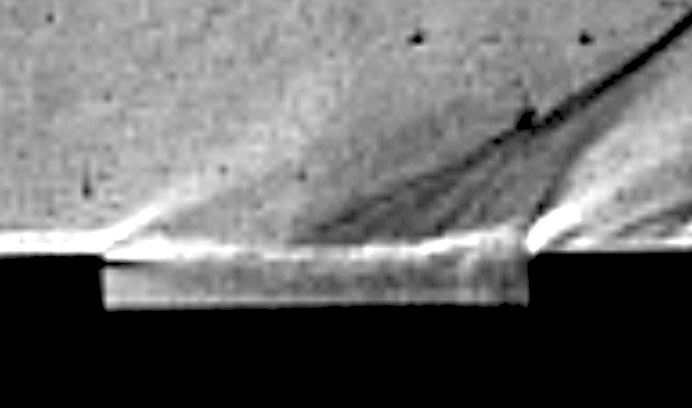
\includegraphics[width = \textwidth]{Figures/9.jpg}
\caption[Schlieren image of cavity. L/D = 9.]{Schlieren image of cavity. L/D = 9.}
\label{fig:9}
\end{figure}

\begin{sidewaysfigure}[p!]
\centering
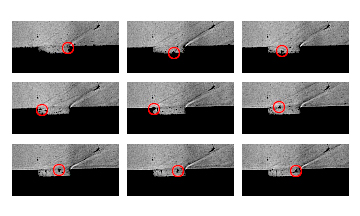
\includegraphics[width = \textwidth]{Figures/cavResTime.jpg}
\caption[Time-correlated Schlieren image of cavity. L/D = 5.]{Time-correlated Schlieren image of cavity. L/D = 5. 9 frames out of 68 are shown. Residence time = 850 $\mu$s.}
\label{fig:ResTime}
\end{sidewaysfigure}
\clearpage

\begin{figure}
\centering
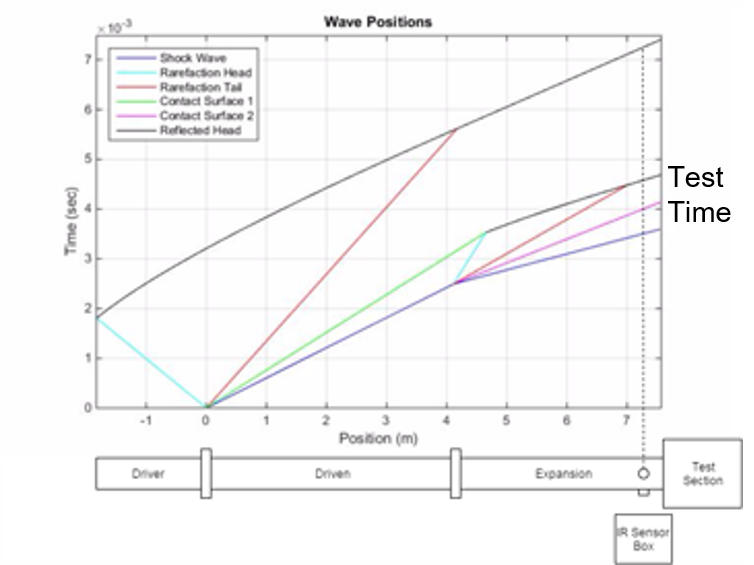
\includegraphics[width = \textwidth]{Figures/XTDiag.png}
\caption[X-T Diagram of Cavity Tests]{X-T diagram generated from the initial conditions of the cavity tests: P4 = 225psi, P1 = 0.5psi, P$_e$ = 0.25psi. The test gas was nitrogen.}
\label{fig:XT}
\end{figure}

\begin{figure}
\centering
\includegraphics[width = \textwidth]{Figures/CO2-2.jpg}
\caption[IR Signal for Test 046]{IR Signal for Test 056. P4 = 225psi, P1 = 0.5psi, P$_e$ = 0.25psi. The test gas was a 95\% nitrogen and 5\% CO$_2$ mixture. Test Time = 434 $\mu$s.}
\label{fig:IRTrace}
\end{figure}

\begin{figure}
\centering
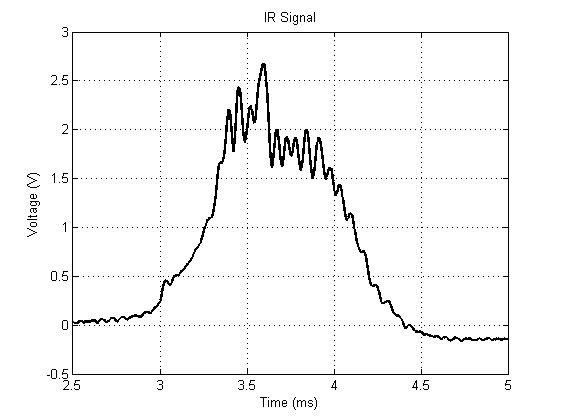
\includegraphics[width = \textwidth]{Figures/H2.jpg}
\caption[IR Signal for Test 046]{IR Signal for Test 057. P4 = 225psi, P1 = 0.75psi, P$_e$ = 0.25psi. The test gas was a hydrogen and oxygen mixture followed by a 95\% nitrogen and 5\% CO$_2$ mixture. Test Time = 561 $\mu$s.}
\label{fig:IRTrace2}
\end{figure}

\begin{figure}
\centering
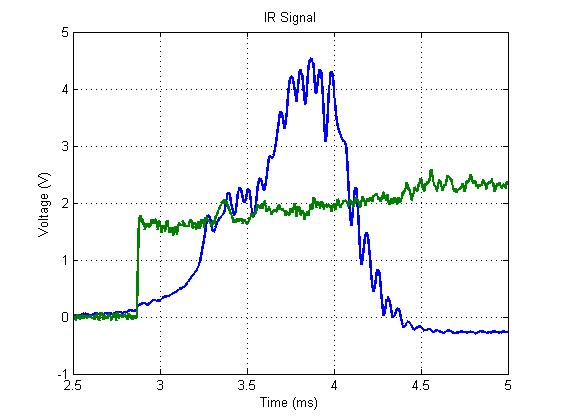
\includegraphics[width = \textwidth]{Figures/H2andCo2.jpg}
\caption[IR Signal for Test 046]{IR Signal for Test 058. P4 = 225psi, P1 = 0.5psi, P$_e$ = 0.25psi. The test gas was a 95\% Nitrogen and 5\% CO$_2$ mixture. Test Time = 333 $\mu$s.}
\label{fig:IRTrace3}
\end{figure}

 
%% Chapter Template

\chapter{Future Work} % Main chapter title

\label{Chapter6} % Change X to a consecutive number; for referencing this chapter elsewhere, use \ref{ChapterX}

\lhead{Chapter 6. \emph{Future Work}} % Change X to a consecutive number; this is for the header on each page - perhaps a shortened title

%----------------------------------------------------------------------------------------
%	SECTION 1
%----------------------------------------------------------------------------------------

\section{Phase 3}




%----------------------------------------------------------------------------------------
%	SECTION 2
%----------------------------------------------------------------------------------------

\section{Suggestions for Other Improvements}
 

%----------------------------------------------------------------------------------------
%	THESIS CONTENT - APPENDICES
%----------------------------------------------------------------------------------------

\addtocontents{toc}{\vspace{2em}} % Add a gap in the Contents, for aesthetics

\appendix % Cue to tell LaTeX that the following 'chapters' are Appendices

% Include the appendices of the thesis as separate files from the Appendices folder
% Uncomment the lines as you write the Appendices

% Appendix A

\chapter{Implementation and Troubleshooting of the Timer Counter Circuit} % Main appendix title

\label{Appendix 1} % For referencing this appendix elsewhere, use \ref{AppendixA}

When using the timer counter box, make sure the box is plugged into the power supply. Once the box has power, turn on the power supply associated with the inverting circuit. Once these are powered, the blue amplifier boxes should be turned on to supply power to the transducers. Set the appropriate gains on these boxes. The appropriate gains are based on what magnitude signal is desired. The LabVIEW program will only read signals between 0 and 5V. The pressure transducers output 0-5V for a pressure range of 0 to 100 psi. However, the pressure these transducers will be exposed to are only between 10 and 20 psi, resulting in a 0.5 to 1V signal. Setting the gain to 5 allows that signal to be amplified to to between 2.5 and 5V. Having a larger signal allows for the comparator circuit to operate more easily. One can set the comparator nominal voltage with confidence, as the larger signal allows for a larger margin of error on the set comparator voltage. This gives more confidence that the signal coming into the comparator circuit will be large enough to trigger a digital signal. 

Once the physical systems are powered and ready, run the two LabVIEW programs for the capturing of the digital signals as well as the analog signals. The analog program filename is ''BasicHighSpeedOscillosope-fixed.vi'' and the digital program filename is ''CountersWorking.vi'' For the analog signal, an input is required for sampling rate and time to take data. The typical sampling rate and time for tests is 1MHz and 10,000 $\mu$s. The digital program asks for a user input of ''milliseconds to wait.'' This is the amount of time the program should wait until sending the 5V TTL pulse to the camera. Typically, this value is set to 0. 

One common problem with this circuit is that no digital signal is sent from the circuit itself. To check for this, use a function generator and an oscilloscope. Hook up the oscilloscope to one of the digital out wires of the box as well as the output of the function generator. Table \ref{Table:pins} shows the number of the digital out wire to its corresponding number. Attach the function generator to the corresponding BNC connector. A T-connector is needed to split the output signal from the function generator. Send a 5V amplitude sine wave from the function generator. The corresponding signal from the box should be a square wave. If there is no square wave present, check that the potentiometer is not too high or too low. The square wave should get wider or narrower depending on the position of the potentiometer. If there is still no signal coming from the box, there may be a burnt out op-amp. If, however, there is no signal coming from any of the outputs, it is unlikely all of the op-amps burned out. In this case, there may be a wiring issue. For this, check continuity between the signal coming in and the signal coming out to make sure voltages at each connection are what they are supposed to be. Some alteration of the circuit may be required in this case. However, that is unlikely, and the problem is likely to be that the potentiometer level was set too high.

\begin{table}[]
\centering
\caption[Digital Pin Out Colors]{Digital Out Pin Colors on the comparator circuit box corresponding to their Analog In numbers}
\label{Table:pins}
\begin{tabular}{l|l}

Analog In & Digital Out \\ \hline
1        & Blue       \\ 
2        & Purple     \\ 
3        & Black       \\ 
4        & Yellow       \\ 
5 		 & White		\\
6 		 & Red	      \\
GND      & Green	\\
Extra    & Orange	\\
\end{tabular}
\end{table}

\lhead{Appendix A. \emph{Timer Counter Setup and Troubleshooting}} % This is for the header on each page - perhaps a shortened title

%% Appendix B

\chapter{Implementation of the IR Sensor} % Main appendix title

\label{Appendix 2} % For referencing this appendix elsewhere, use \ref{AppendixA}

To achieve the sensitivity required for the sensor, the operating temperature of the IR detector is about 77K, and the detector must be cooled with liquid nitrogen. Using the funnel to avoid spillage of the liquid nitrogen onto the cable connections or viewing window of the sensor, a few hundred milliliters were poured into the hole at the top of the sensor. When the sensor reaches the correct temperature, an eruption of cool gas occurs. It is important to wait until this eruption completes because the buildup of gas can cause the cap to blow off. Once the eruption subsides, the cap can be replaced to the top of the sensor and power can be supplied to the amplifier. 

The amplifier can be utilized in two settings, AC or DC coupled. AC coupling, uses an extra capacitor to filter the DC component out of a signal containing both AC and DC elements. DC coupling allows for both the AC and DC elements to pass. The main consideration for the IR sensor, though is the gain present at each of the coupling settings. AC coupling introduces a 10x gain to the signal, which is useful, as the level of the emission signal is relatively low, at less than 0.5V. Although DC coupling could be utilized, the gain on the amplifier provides a stronger signal to analyze. For typical IR emission tests, be sure the amplifier is set to AC coupled. If the IR sensor is to be run in absorption mode with the IR light source, DC coupling should be used, as the light source provides a relatively large base signal. To switch between AC and DC coupling, simply plug the cable that goes between the amplifier and the IR sensor into the appropriately labeled spot on the amplifier.

After power is supplied to the sensor through the amplifier, it is important to check that the system is aligned. Since the setup is attached to the support structure and not the tube itself, the recoil of the tube or the moving of the tube to replace diaphragms can alter the alignment of the window to the focusing mirror. To re-align the system, a stainless steel LED tube was constructed. This tube fits within the porthole on the back side of the tube, aligned with the port for the IR sensor. With the LED on and lined up with the inside wall of the far side of the tube, check the light source path. Be sure that the thin slit of red light hits the small sensor area. Adjust the flat mirror as needed to align the slit of red light with the IR sensor pickup area. Once the system is aligned, remove the LED tube and replace the plug in that port. The system at this point is aligned and ready for a test.  

\lhead{Appendix B. \emph{IR Sensor Setup}} % This is for the header on each page - perhaps a shortened title

%% Appendix B

\chapter{IR Test Information} % Main appendix title

\label{Appendix 3} % For referencing this appendix elsewhere, use \ref{AppendixA}
\begin{table}[h!]
\centering
\caption{Basic pressure, timer counter, IR, and test time data from all successful tests utilizing the IR sensor. The test gas labeled CO$_2$ was a 5\% CO$_2$ mixture in nitrogen. The test gas labeled H$_2$ was a 2H$_2$ + O$_2$ + 8N$_2$ mixture. *Staged filling resulted in two levels of IR signal. The first number represents the time the Hydrogen mixture passed the sensor, while the second represents the CO$_2$ mixture.}

\label{IRinfo}
\begin{tabular*}{\textwidth}{|l|
>{\columncolor[HTML]{EFEFEF}}l l
>{\columncolor[HTML]{EFEFEF}}l l
>{\columncolor[HTML]{EFEFEF}}l l
>{\columncolor[HTML]{EFEFEF}}l l
>{\columncolor[HTML]{EFEFEF}}l |}
\hline
Test No.      & \textbf{041}  & \textbf{046}  & 0\textbf{47}  & \textbf{049}  & \textbf{050}  & \textbf{055}    & \textbf{056}    & \textbf{057}        & \textbf{058}         \\ \hline
Test Gas      & N$_2$   & N$_2$   & N$_2$   & N$_2$   & N$_2$   & CO$_2$ & CO$_2$ & H$_2$ & Staged \\ \hline
P4 (psi)      & 225  & 225  & 225  & 225  & 226  & 225    & 224    & 225        & 223         \\ \hline
P1 (psi)      & 0.5  & 0.51 & 0.5  & 0.5  & 0.75 & 0.51   & 0.5    & 0.75       & 0.76        \\ \hline
Pe (psi)      & 0.5  & 0.25 & 0.25 & 0.25 & 0.25 & 0.26   & 0.26   & 0.28       & 0.25        \\ \hline
T1 (s)        & 189  & 210  & N/A  & N/A  & N/A  & 223.4 & 205.9 & 184.9    & 903.2      \\ \hline
T2 (ms)       & 2.47 & N/A  & N/A  & N/A  & N/A  & 1.73 & 1.67 & 1.7733     & 1.67      \\ \hline
T3 (s)        & 147  & N/A  & N/A  & N/A  & N/A  & 157.7 & 147.2 & 170.4      & 150.5      \\ \hline
T4 (s)        & 148  & 153  & N/A  & N/A  & N/A  & 160.1  & 150.9 & 171.3     & 150.0      \\ \hline
IR Time (s)   & 467  & 399  & 466  & 436  & 424  & 429    & 434    & 561        & 333, 473*  \\ \hline
Test Time (s) & 363  & 551  & 544  & 544  & 659  & 544    & 538    & 676        & N/A         \\ \hline
\end{tabular*}
\end{table}



\lhead{Appendix C. \emph{IR Test Information}} % This is for the header on each page - perhaps a shortened title


\addtocontents{toc}{\vspace{2em}} % Add a gap in the Contents, for aesthetics

\backmatter

%----------------------------------------------------------------------------------------
%	BIBLIOGRAPHY
%----------------------------------------------------------------------------------------

\label{Bibliography}

\lhead{\emph{Bibliography}} % Change the page header to say "Bibliography"

\bibliographystyle{unsrtnat} % Use the "unsrtnat" BibTeX style for formatting the Bibliography

\bibliography{Bibliography} % The references (bibliography) information are stored in the file named "Bibliography.bib"

\end{document}  